\documentclass[a4paper, toc=index, 12pt, DIV14, twoside, BCOR2cm, headsepline, numbers=noenddot, bibliography=totoc]{scrbook}

\usepackage{tikz} 
\usetikzlibrary{shapes,arrows}
\usepackage[utf8]{inputenc}
\usepackage[T1]{fontenc}
\usepackage[american,ngerman]{babel}	% Choose languages here. This affects the section naming as well, like "Abstract" in EN and "Zusammenfassung" in DE.


% CUSTOM
\usepackage[colorinlistoftodos,prependcaption,textsize=normalsize]{todonotes}
%\newcommandx{\unsure}[2][1=]{\todo[linecolor=red,backgroundcolor=red!25,bordercolor=red,#1]{#2}}
%\newcommandx{\change}[2][1=]{\todo[linecolor=blue,backgroundcolor=blue!25,bordercolor=blue,#1]{#2}}
%\newcommandx{\info}[2][1=]{\todo[linecolor=OliveGreen,backgroundcolor=OliveGreen!25,bordercolor=OliveGreen,#1]{#2}}
%\newcommandx{\improvement}[2][1=]{\todo[linecolor=Plum,backgroundcolor=Plum!25,bordercolor=Plum,#1]{#2}}
\usepackage[T1]{fontenc}
\usepackage{lmodern}
\usepackage[hyphens]{url}
\usepackage{threeparttable}

% END CUSTOM


\usepackage{ifthen} 
\newboolean{bachelorThesis}
\newboolean{labProject}
\newboolean{masterThesis}
 
%% Enter thesis type here ("Master Thesis", "Lab Project", "Bachelor Thesis") and set boolean variables accordingly.
\setboolean{bachelorThesis}{false}
\setboolean{masterThesis}{false}
\setboolean{labProject}{true}
 
\newcommand{\thesisTitle}{Smart Heating System\\ in Residential Areas}

% BSC thesis 
\ifthenelse{\boolean{bachelorThesis}}
{
\newcommand{\thesisType}{Bachelor Thesis}
\newcommand{\thesisAuthor}{Student Name} 
\newcommand{\thesisETHID}{XX-XXX-XXX}
\newcommand{\thesisEmail}{student@student.ethz.ch}
}{}

% MS thesis
\ifthenelse{\boolean{masterThesis}}
{
\newcommand{\thesisType}{Master Thesis}
\newcommand{\thesisAuthor}{Student Name}
\newcommand{\thesisETHID}{XX-XXX-XXX}
\newcommand{\thesisEmail}{student@student.ethz.ch}
}{}

% Lab project
\ifthenelse{\boolean{labProject}}
{
\newcommand{\thesisType}{Lab Project}
\newcommand{\thesisAuthorI}{Michael Spiegel}
\newcommand{\thesisAuthorII}{Samuel Schmid}
\newcommand{\thesisAuthor}{\thesisAuthorI \\and \thesisAuthorII}
\newcommand{\thesisETHID}{10-915-312 (\thesisAuthorI)\\[1mm] & 10-919-991 (\thesisAuthorII)}
\newcommand{\thesisEmail}{spiegelm@student.ethz.ch\\[1mm] & schmisam@student.ethz.ch}
}{}


\newcommand{\thesisSemester}{Spring 2015}
\newcommand{\thesisSubmission}{\color{red}TODO}
%\newcommand{\thesisSubmission}{January 5, 2012}

\usepackage{amsmath,amsfonts,amssymb}
\usepackage{graphicx}
\usepackage[plainpages=false,pdfpagelabels,bookmarks=true,backref=false,pagebackref=false]{hyperref}
\usepackage[tracking=true]{microtype}
\usepackage[nice]{nicefrac}
\usepackage{booktabs}
\usepackage{float}
\usepackage{flafter}
\usepackage{makeidx}
\usepackage{cite}
\usepackage{color}
\usepackage{wrapfig}
\usepackage{tabularx}
\usepackage{multicol}
\usepackage{paralist}
\usepackage{graphics}

\hypersetup{ 
	pdfauthor={\thesisAuthor},
	pdftitle={\thesisTitle},
	pdfsubject={\thesisType},
	colorlinks=false,
	breaklinks=true,
	pdfborder=0 0 0,
	citebordercolor=0 0 0,
	filebordercolor=0 0 0,
	linkbordercolor=0 0 0,
	menubordercolor=0 0 0,
	urlbordercolor=0 0 0,
	pdfhighlight=/I,
	bookmarksopen=false,
	bookmarksnumbered=true
}

\usepackage{listings}
\lstloadlanguages{C}
\lstset{numbers=left, numberstyle=\tiny, numbersep=5pt, language=C, basicstyle=\ttfamily\scriptsize, tabsize=2, breaklines=true}

% Disable single lines at the start of a paragraph (Schusterjungen)
\clubpenalty = 10000

% Disable single lines at the end of a paragraph (Hurenkinder)
\widowpenalty = 10000 \displaywidowpenalty = 10000

\renewcommand{\topfraction}{1.0}    % Bilder duerfen auch direkt am
                                    % Seitenanfang sein
\renewcommand{\bottomfraction}{1.0} % Bilder duerfen auch direkt am
                                    % Seitenende sein







% CUSTOM SECTION


%\makeatletter
%\newcommand{\figsourcefont}{\footnotesize}
%\newcommand{\figsource}[1]{%
%  \addtocontents{lof}{%
%    {\leftskip\cftfigindent
%     \advance\leftskip\cftfignumwidth
%     \rightskip\@tocrmarg
%     \figsourcefont#1\protect\par}%
%  }%
% }
%\makeatother


\linespread{1.1}
\setlength{\parskip}{10pt}

\setcounter{secnumdepth}{3} % numbering of subsubsections
\setcounter{tocdepth}{3}	% includes subsubsections in the table of contents


\usepackage{booktabs}

% in place code
\lstnewenvironment{code}[1][]%
{
   \noindent
   \minipage{\linewidth} 
   \vspace{0.5\baselineskip}
   \lstset{basicstyle=\ttfamily\footnotesize,#1}}
{\endminipage}

% floating code
\lstnewenvironment{snippet}[1][]
    {\lstset{float=htpb,#1}} 
    {}

\usepackage{caption}
\captionsetup{labelfont={sf,bf},font=footnotesize,format=plain}

\usepackage{enumitem}

% Taken from Lena Herrmann at 
% http://lenaherrmann.net/2010/05/20/javascript-syntax-highlighting-in-the-latex-listings-package
%\documentclass{article}
%\usepackage{listings}
%\usepackage{color}
\definecolor{lightgray}{rgb}{.9,.9,.9}
\definecolor{darkgray}{rgb}{.4,.4,.4}
\definecolor{purple}{rgb}{0.65, 0.12, 0.82}

\lstdefinestyle{nolinenumbers}
{
	numbers=none,
	backgroundcolor=\color{white}
}

% END CUSTOM SECTION



\makeindex


\begin{document}

\frontmatter

\begin{titlepage}

	\flushleft
	
	\vspace*{-20mm}
	{
		
\includegraphics[width=5cm]{images/logos/logo_ETH} 
		\hfill
		
\includegraphics[width=5cm]{images/logos/logo_DSG}
	}
	  
  \vfill
  \vfill

  	{\Huge \sffamily \bfseries \thesisType}\\[3mm]Institute for Pervasive Computing, Department of Computer Science, ETH Zurich
  	\rule{\textwidth}{1mm}
  
  \vfill
	
	\begin{center}
	 		\Huge \sffamily \bfseries
	 		\thesisTitle
 	\end{center}
 	
 	\vspace{10pt}
 	
 	\begin{center}
 		\Large
  		by \thesisAuthor
	
 	\end{center}
 	
 	\vspace{10pt}
  
  \begin{center}
 		\Large
 		\thesisSemester
 	\end{center}
  
  \vfill
  \vfill
  \vfill
  
  	\setlength{\tabcolsep}{0mm}
		\begin{tabular}{p{40mm}l}
			ETH student ID:     & \thesisETHID \\[1mm]
			E-mail address:     & \thesisEmail \\[5mm]
			Supervisors:        & Dr. Wilhelm Kleiminger\\[1mm]
			                    & Prof. Dr. Friedemann Mattern\\[5mm]
			Date of submission: & \thesisSubmission
		\end{tabular}
	
\end{titlepage}

\thispagestyle{empty}
\begin{center}
\parbox{0mm}{}
\end{center}
% \parskip 10pt

\chapter*{Declaration of Originality}

I hereby declare that this written work I have submitted is original work which
I alone have authored and which is written in my own words.
\\
With the signature I declare that I have been informed regarding normal academic citation rules
and that I have read and understood the information on ``Citation etiquette'':
\begin{center}
\url{http://www.ethz.ch/students/exams/plagiarism_s_en.pdf}
\end{center}
The citation conventions usual to the discipline in question here have been
respected.
\\
This written work may be tested electronically for plagiarism.

\vspace{3cm}

\ifthenelse{\boolean{labProject}}
{
\noindent
{
\begin{minipage}[t]{6cm}
	Zurich, \thesisSubmission
\end{minipage}\hfill
\begin{minipage}[t]{6cm}
	%\phantom{M}\\
	\vskip 12pt
	\rule{6cm}{0.5pt} \\
	\parbox{6cm}{\hfill \thesisAuthorI \hfill\vbox{}}
\end{minipage}\hfill
}

\vspace{3cm}

\noindent
{
\begin{minipage}[t]{6cm}
	~
\end{minipage}\hfill
\begin{minipage}[t]{6cm}
	%\phantom{M}\\
	\vskip 12pt
	\rule{6cm}{0.5pt} \\
	\parbox{6cm}{\hfill \thesisAuthorII \hfill\vbox{}}
\end{minipage}\hfill
}
}
{
\noindent
{
\begin{minipage}[t]{6cm}
	Zurich, \thesisSubmission
\end{minipage}\hfill
\begin{minipage}[t]{6cm}
	%\phantom{M}\\
	\vskip 12pt
	\rule{6cm}{0.5pt} \\
	\parbox{6cm}{\hfill \thesisAuthor \hfill\vbox{}}
\end{minipage}\hfill
}
}



%!TEX root = ../thesis.tex

\selectlanguage{american} % american ngerman
\chapter*{\abstractname}
\label{chap:abstract}

In this lab project we present a reliable heating control system for residential users.
This project consists of two major parts.
On the one hand there is the back end consisting of the local infrastructure monitoring and controlling temperatures and persisting this data on an accessible web server.
On the other hand there is the front end as an Android mobile application offering a user friendly interface to configure and control the system. The application is a lightweight distributed software system designed for multiple users in the same residence.
%%!TEX root = ../thesis.tex

\chapter*{Acknowledgements}
If you want, put some acknowledgements here.

\tableofcontents

\mainmatter

%!TEX root = ../thesis.tex

\chapter{Introduction}
\label{sec:introduction}

% Motivate your problem and outline the contributions of the thesis.\cite{mattern2010ict}

%As energy consumption is growing world wide, the need for technologies to control and analyze energy consumption increases.
%Therefore a lot of tools exist, that show the energy consumption of a household, business or certain devices. 
%But most of these technologies and tools are very complex for the end user, as most of the times the user is not a domain expert.

The energy consumption is growing world wide and causes increasing costs and environmental damage.
In 2010, private households in Switzerland consumed 30\% of the total energy, most of it for heating purposes\cite{x}.
A lot of different tools in the domain of residential heating control were developed to help reducing the consumed energy for space heating.
But most of these tools do either not motivate end users to save energy or are too complex to use for the end user and thus discarded in the long-term.
This results in the need of user friendly tools that provide the end user with enough information to analyze their data but not overwhelm him with unnecessary details.

%One of the areas in which easy to use tools are needed, is heating control.
%For this specific area we developed our project, which consists of two parts: the infrastructure and the mobile application.
%The infrastructure part gets the heating data and analyzes it while the mobile application provides an easy to use and well understandable visualization of the data.

For this specific area we developed our project, which consists of a reliable infrastructure serving as a solid base, and a well designed mobile application allowing the user to configure and interact with the system.

This report is structured as follows.
Chapter~\ref{sec:relatedwork} outlines previous work done in fields related to this thesis.
Chapter~\ref{sec:requirements} treats the process of determining the requirements of the infrastructure and applications developed in the scope of this lab project.
Chapter~\ref{sec:systemoverview} gives an overview of the whole system environment and introduces the chosen architecture of our application.
Chapter~\ref{sec:infrastructure} explains the developed infrastructure with the local deployment and the communication server in detail.
Chapter~\ref{sec:mobile_app} describes the implemented mobile application in detail.
In Chapter~\ref{sec:evaluation} we evaluate the developed system considering the defined requirements and design goals.




%%!TEX root = ../thesis.tex

\chapter{Related Work}
\label{sec:relatedwork}

Put related work here~\cite{mattern2010ict}.

CoAP, REST

wenig wissenschaftlich: Django, Android
%!TEX root = ../thesis.tex

\chapter{Requirements Elicitation}
\label{sec:requirements}

\section{Functional Requirements}

Functional requirements are stated using use cases in the style of Martin Fowler\footnote{\url{http://en.wikipedia.org/wiki/Use_case\#Fowler_style}}\footnote{\url{http://ontolog.cim3.net/cgi-bin/wiki.pl?UseCasesMartinFowlerSimpleTextExample}}. Each use case is described by stating the main goal of the use case in its title, followed by the main success scenario as a list of steps. After that we list a series of extensions which describe a condition that leads to a different interaction depending on user input or the system's state.


\subsection{Register a Residence}
User has bought the smart heating system and would like to register his residence.
\begin{enumerate}
    \item User opens the app and opens the registration screen
    \item User scans the RFID tag\footnote{Every element of the system is equipped with an RFID tag (Radio-frequency identification). More about this can be found in Section \ref{sec:server_infrastructure_models}.}
    \item System checks if RFID is not yet registered
    \item System registers residence with scanned RFID
    \item App shows empty home screen with no rooms
\end{enumerate}

\paragraph{Alternative} RFID already registered or invalid
\begin{itemize}
    \item At step 3, system fails to verify that RFID is not yet registered
    \item{If RFID is associated to a residence
        \begin{itemize}
        \item App shows the home screen of the registered residence
        \end{itemize}
        }
    \item {If RFID is associated to a thermostat
        \begin{itemize}
        \item App shows error message telling the user that he needs to scan the Raspberry Pi instead of a thermostat
        \item Return to primary scenario at step 2
        \end{itemize}
    }
    \item {If RFID is invalid
        \begin{itemize}
        \item App shows error message telling the user that he needs to scan a valid RFID
        \item Return to primary scenario at step 2
        \end{itemize}
    }
\end{itemize}
    
\paragraph{Alternative} NFC Adapter\footnote{A Near Field Communication adapter is necessary to allow the user's phone to scan the RFID tags on the elements of the system.} not available
\begin{itemize}
    \item 1a. App shows a manual scan button
    \item 1b. User taps the manual scan button and enters the RFID on the tag by hand
    \item Return to primary scenario at step 3
\end{itemize}

\subsection{Add a Room to a Residence}
User has already registered his residence and would like to add rooms to the home screen.
\begin{enumerate}
    \item User opens the app and opens the home screen
    \item User taps the Add Room button
    \item User is prompted for a name for the new room
    \item System registers a new room with the given name 
    \item App shows home screen with the newly added room
\end{enumerate}

\paragraph{Alternative} Invalid name entered
\begin{itemize}
    \item At step 3, the user has entered an empty name
    \item App notifies user that the name must be entered and allows him to retry
    \item Return to primary scenario at step 3
\end{itemize}

\subsection{Add a Thermostat to a Room}
User is still setting up his system and has just added a room. He would like to register the thermostats in the current room.
\begin{enumerate}
    \item User opens the app and opens the home screen
    \item User taps on the room he would like to add a thermostat to
    \item User scans the RFID tag
    \item System checks if RFID is not yet registered
    \item App shows the room's detail view with the newly added thermostat
\end{enumerate}

\paragraph{Alternative} RFID already registered or invalid
\begin{itemize}
    \item At step 3, system fails to verify that RFID is not yet registered
    \item{If RFID is associated to a residence
        \begin{itemize}
        \item App shows error message telling the user that he needs to scan the  thermostat instead of the Raspberry Pi
        \item Return to primary scenario at step 3
        \end{itemize}
        }
    \item {If RFID is associated to an already registered thermostat
        \begin{itemize}
        \item App shows error message telling the user that each thermostat can only be registered to a single room and tells him what room the scanned thermostat belongs to
        \item Return to primary scenario at step 3
        \end{itemize}
    }
    \item {If RFID is invalid
        \begin{itemize}
        \item App shows error message telling the user that he needs to scan a valid RFID
        \item Return to primary scenario at step 3
        \end{itemize}
    }
\end{itemize}

\paragraph{Alternative} NFC Adapter not available
\begin{itemize}
    \item 2a. App shows a manual scan button
    \item 2b. User taps the manual scan button and enters the RFID on the tag by hand
    \item Return to primary scenario at step 4
\end{itemize}

\subsection{Heat up a Room}
User is sitting in his living room and feels cold. He would like to use his new smart heating system to heat up the room.
\begin{enumerate}
    \item User opens the app and opens the home screen
    \item User taps the room icon for the living room
    \item User checks the currently set temperature for the room
    \item User changes the target temperature of the room to a higher value
    \item System checks if the entered temperature is in a valid range
    \item System changes the target temperature for the thermostats associated for the room
    \item Thermostats start heating the room
\end{enumerate}

\paragraph{Alternative} Invalid temperature entered
\begin{itemize}
    \item At step 4, the user has entered an invalid temperature value
    \item App notifies user that the temperature must be in a certain range and allows him to retry
    \item Return to primary scenario at step 4
\end{itemize}


\subsection{Cool down a Room}
User is sitting in his office and feels hot. He would like to use his new smart heating system to turn off the heating.
\begin{enumerate}
    \item User opens the app and opens the home screen
    \item User taps the room icon for the living room
    \item User checks the currently set temperature for the room
    \item User changes the target temperature of the room to a lower value
    \item System checks if the entered temperature is in a valid range
    \item System changes the target temperature for the thermostats associated for the room
    \item Thermostats stop heating the room
\end{enumerate}

\paragraph{Alternative} Invalid temperature entered
\begin{itemize}
    \item At step 4, the user has entered an invalid temperature value
    \item App notifies user that the temperature must be in a certain range and allows him to retry
    \item Return to primary scenario at step 4
\end{itemize}

\subsection{Remove a Room from the Residence}
User has already set up the system for all the rooms in his home but has made changes to his house. To accommodate for these changes he needs to remove some rooms from the system.
\begin{enumerate}
    \item User opens the app and opens the home screen
    \item User taps the room icon for the room to be deleted
    \item User taps the delete room button
    \item App prompts the user for confirmation
    \item System removes room and all its associated thermostats
    \item App shows home screen with the deleted room removed
\end{enumerate}

\subsection{Remove a Thermostat from a Room}
One of the thermostats in the user's home has broken down. He buys a new one from the store and wants to replace the old one in the system. After adding the newly bought thermostat he would like to remove the old one from the system.
\begin{enumerate}
    \item User opens the app and opens the home screen
    \item User taps the room icon for the room to be changed
    \item User taps the delete button on the thermostat in question
    \item App prompts the user for confirmation
    \item System removes the thermostat from the room
    \item App shows the room's detail screen with the remaining thermostats (if any)
\end{enumerate}

\subsection{Change a Room's Heating Schedule}
User has noticed that the living room is often still heating up while he is out for work. He would like to change the heating schedule to stop heating when he leaves the house.
\begin{enumerate}
    \item User opens the app and opens the home screen
    \item User taps the room icon for the living room
    \item User taps the change schedule button
    \item App shows the heating schedule for the living room
    \item User changes the schedule, setting the desired heating times
    \item System changes the schedules and sends the update to the Raspberry Pi
\end{enumerate}

\section{Non-Functional Requirements}

\begin{itemize}
    \item \textbf{Extensibility}
    
    Since the development of such a smart heating system usually takes several years with a much larger group than just two people, one of our non-functional requirements is that these applications that we provide in the end should be extensible and can be continued to work on. For more ideas and features that came to mind during development but were not implemented yet, see Section \ref{sec:futurework}.
    \item \textbf{Reliability and Robustness}
    
    As mentioned before, most of the existing systems are either not used properly or even discarded after a while because they are too complex. Since we are aiming for a service that is easy to use and will stay in the user's home for a long time, we want to produce a system that is reliable and robust.
    \item \textbf{Backup}
    
    If the user changes phones, or even has to exchange vital elements of the system, he should not have to reinstall the whole system but rather can only exchange these elements and continue the service without any repercussions.
    
    \item \textbf{Usability}
    
    We want the user to enjoy working with the heating system to guarantee a long lasting deployment as well as the user getting all the benefits from it. 
\end{itemize}





%!TEX root = ../thesis.tex

\chapter{System Overview}
\label{sec:systemoverview}

The system consists of two major parts.
First, the back end consisting of the local infrastructure monitoring and controlling temperatures and persisting this data on an accessible web server.
Second, the mobile application offering a user friendly interface to configure and interact with the system.
See Figure~\ref{fig:system_overview} for a graphical overview.

\begin{figure}[h]
\begin{center}
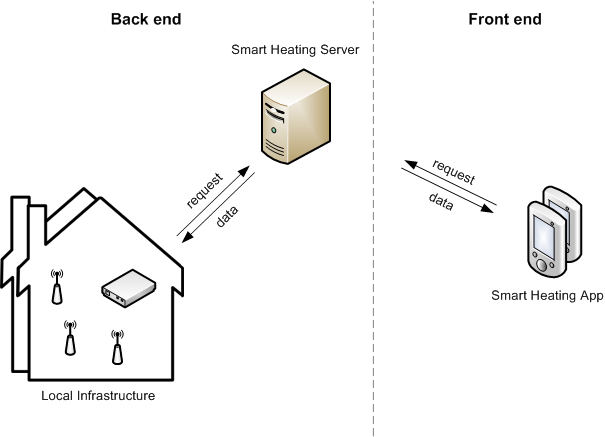
\includegraphics[width=0.9\textwidth]{images/SystemOverview.png}
\end{center}
\caption{
	System overview showing the infrastructure part and the mobile application part.
	The local infrastructure is required for each residence and a residence can be controlled using one or multiple mobile applications.
	The server is required only once and stores the information about all residences.
	}
\label{fig:system_overview}
\end{figure}

The infrastructure part consists of the local residential deployment and the server.
Within the residence a small computer system is installed which serves as a communication gateway to the distributed low-power thermostats.
On the remote side is the server acting as the central entity to collect and store the accumulated sensor data and organizational data.
Both are explained in Chapter~\ref{sec:infrastructure}.

The mobile application part consists of a control application used to communicate between the user and the local infrastructure. It should provide an easy way for the user to control the smart heating system and guide him in installing it in his home. 

\section{Architecture}

The smart heating system is implemented using a server-client model.
% Willi: What does that mean? Describe briefly (in one or two sentences) which functionality is implemented where
The smart heating server hosts a web service acting as an API to provide access to the shared resources.
The local communication gateway uses this API to query the residence configuration and persist the collected measurements.
%The server handles requests from its clients to retrieve or store data.
%A local communication gateway uses this API in two ways.
%First, it queries residence information such as the associated thermostats and the heating schedule.
%Second, it persists the measured temperature data on the server to make it available to other clients.
Complementary, there is the mobile application also acting as a client.
It provides and updates the residence configuration and retrieves sensor data.
%This data is shared to the web server and required sensor data is queried conversely.
%The web server and the local infrastructures form the back end of the whole system whereas the mobile applications running on smart phones represent the front end.
%See Figure~\ref{fig:systemoverview_architecture} for a visual representation.


%\begin{figure}[h]
%	\begin{center}
%		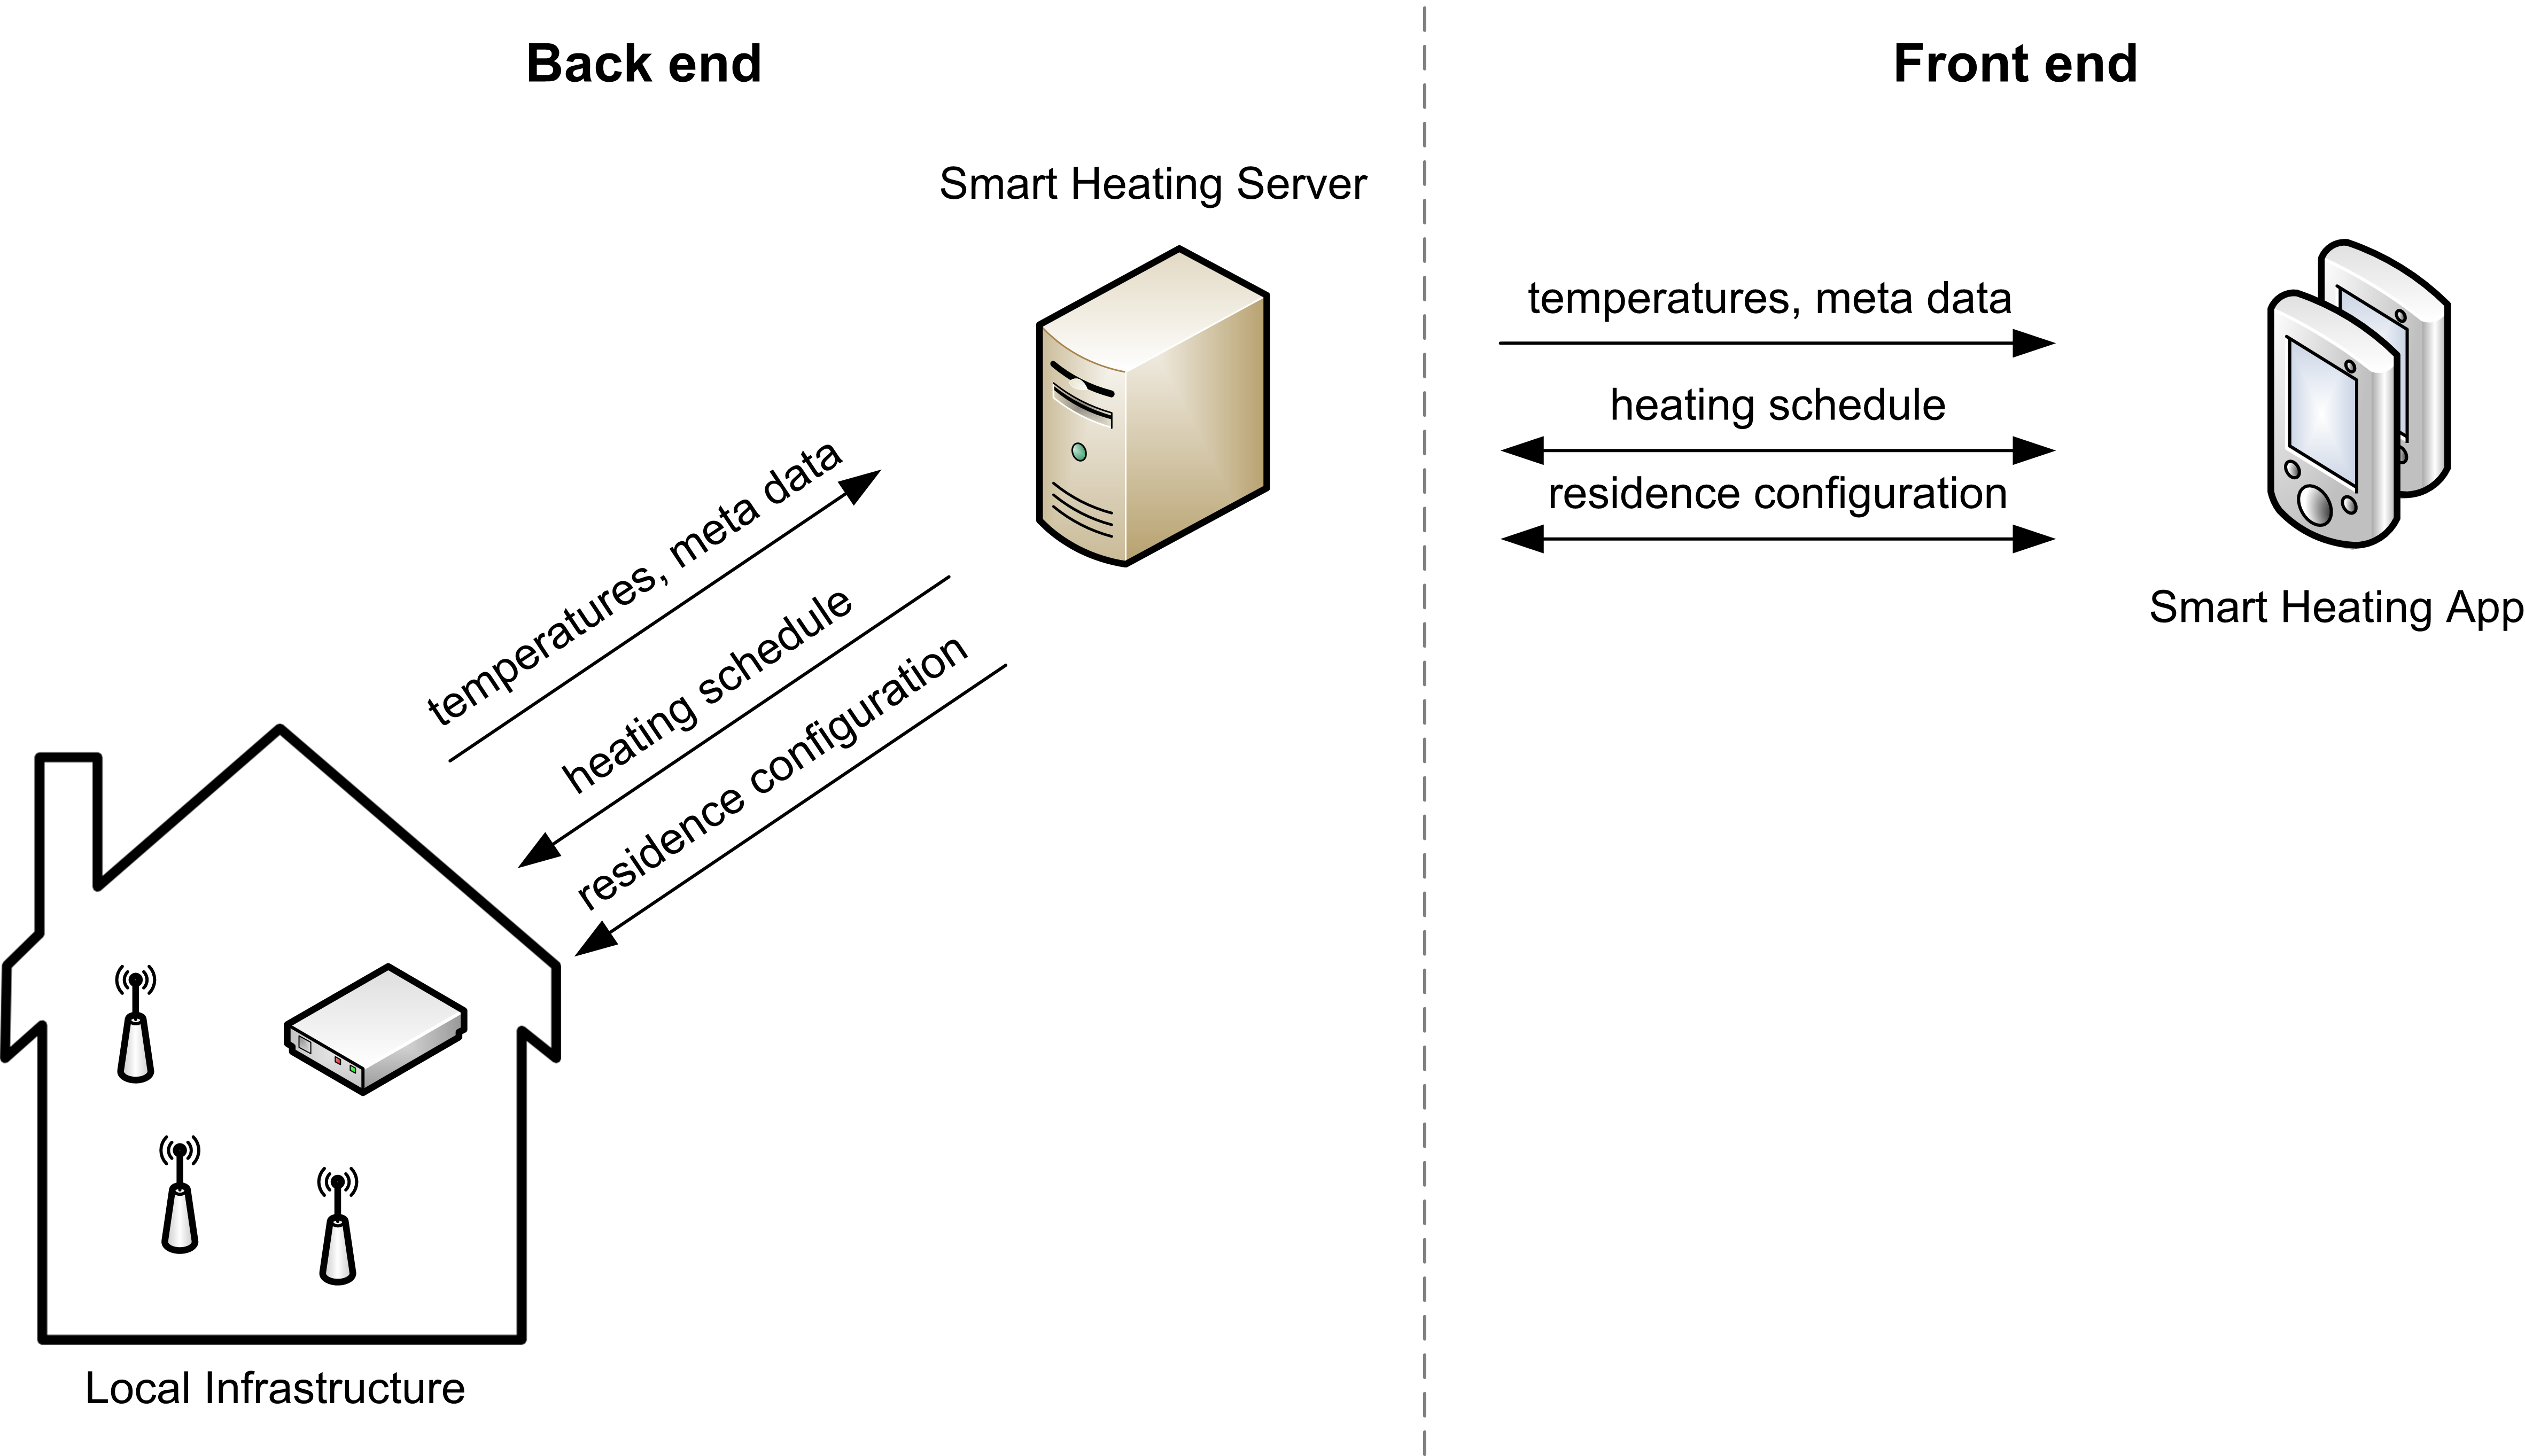
\includegraphics[width=0.95\textwidth]{images/SystemArchitecture.png}
%	\end{center}
%	\caption{Back end and front end depicting the communication between the server and its clients.}
%	\label{fig:systemoverview_architecture}
%\end{figure}


\section{Models}
\label{sec:system_overview_models}

Throughout the project there is a shared system model describing the underlying entities. The system model depicts the physical objects and places that are used for data collection or organizational purposes. The following paragraphs describe the applied models and their associated design decisions.

\paragraph{Residence}

The fundamental unit of each deployment is the residence. Each residence corresponds to an installed local communication gateway. Further details are described in Section~\ref{sec:local_infrastructure}

\paragraph{User}

Each residence can contain multiple users. A user is associated to exactly one residence and is identified by his smart phone IMEI. This design decision simplifies the system design and especially the user authentication. It also prevents a user from using the same identity when accessing the system from multiple smart phones.

\paragraph{Room and Thermostat}
A residence is divided in rooms where each room can contain several thermostats. A room is a simple organizational approach to group multiple thermostats into a single unit.
%Eine Residence ist unterteilt in Räume wobei jeder Raum mehrere Thermostat enthalten kann.

\paragraph{Heating Table}

Each thermostat has an associated temperature schedule called heating table.
The heating table is responsible for mapping each day and time in a week to a target temperature. The heating table is a periodic schedule repeating each week.
This design decision was chosen for infrastructure simplicity as well as to reduce usability complexity.

\paragraph{Meta Entries}

Meta entries persist time depending meta information about thermostats. A meta entry consists of the received signal strength, up-time, battery level and an associated timestamp. This data can be used to identify issues regarding the thermostat devices such as wireless connection problems or drained batteries.
%!TEX root = ../thesis.tex

\chapter{Infrastructure}
\label{sec:infrastructure}

The infrastructure implements a server-client design pattern and is divided into two parts:
The \emph{Server} part and the \emph{Local} part.
First, the server is an independent unit providing a public API to its clients.
Second, the local part is a client consuming the provided API to retrieve configuration from the server and populate it with data gathered from the deployed residential infrastructure.
Both parts will be explained in the following sections.

\section{Server Infrastructure}
\label{sec:server_infrastructure}

The server is the main storage and communication center of this project.
It persists data collected by the local deployment as also organizational information and heating schedules provided by the user via the Mobile App.

\subsection{Design Goals}

\begin{itemize}
\item \emph{Modularity} for independent, interchangeable components for improved Maintainability.
\item \emph{Extensibility} to easily add new resources and relationships.
\item \emph{Usability} for developers.
\item \emph{Testability} for good and comprehensible tests.
\end{itemize}

\subsection{Platform and Frameworks}

The server is implemented with Python, a general-purpose, multi-paradigm programming language\footnote{\url{https://www.python.org/}}.
Python was chosen as it is suitable for developing a solid web server as also for usage on restricted hardware like the Raspberry Pi used for the local deployment.
Django\footnote{\url{https://www.djangoproject.com/}} is a popular web application framework based on a model-view-controller (MVC) pattern facilitating the development of complex, database-driven web applications.
The Django REST Framework\footnote{\url{http://www.django-rest-framework.org/}} extends Django to support the design of RESTful Web APIs.

\subsection{RESTful API}

The server provides a RESTful API designed to persist temperature and heating schedule data of several thermostats.

Each resource is identified by a uniform resource identifier (URI). There are two major types of URIs, resource collections and resource representations.
A resource representation is a view of its resource's state and is usually encoded in XML or JSON.
Resource collections can contain multiple representations of the same type of a resource.

\paragraph{Design Decisions}

\begin{itemize}
    \itemsep0em
    \item Resource collections are referenced per URL. Resources are referenced by including their representation.
    \item URL fields are identified by the name \emph{url} or the suffix \emph{\_url}. Each resource representation contains its own URL in the field \emph{url}.
\end{itemize}

\paragraph{Browsable API}

The Django REST Framework 

Discoverability



\subsection{Program Architecture and Implementation}

The server implementation is built on the Django Framework following a variation\footnote{\url{https://docs.djangoproject.com/en/1.8/faq/general/\#django-appears-to-be-a-mvc-framework-but-you-call-the-controller-the-view-and-the-view-the-template-how-come-you-don-t-use-the-standard-names}} of the Model-View-Controller (MVC) architectural pattern\footnote{\url{https://en.wikipedia.org/wiki/Model-view-controller}}. We assume the user to be familiar with the common MVC pattern.\todo{Explain Djangos architecture?}

\subsubsection{Models}

Models provide an abstraction layer for structuring and manipulating data handled by the web application\todo[fancyline]{Rewrite this sentence, less copying.}.
% A high level description of all used models is given in Section~\ref{sec:system_overview_models}. 

\begin{figure}[h]
\begin{center}
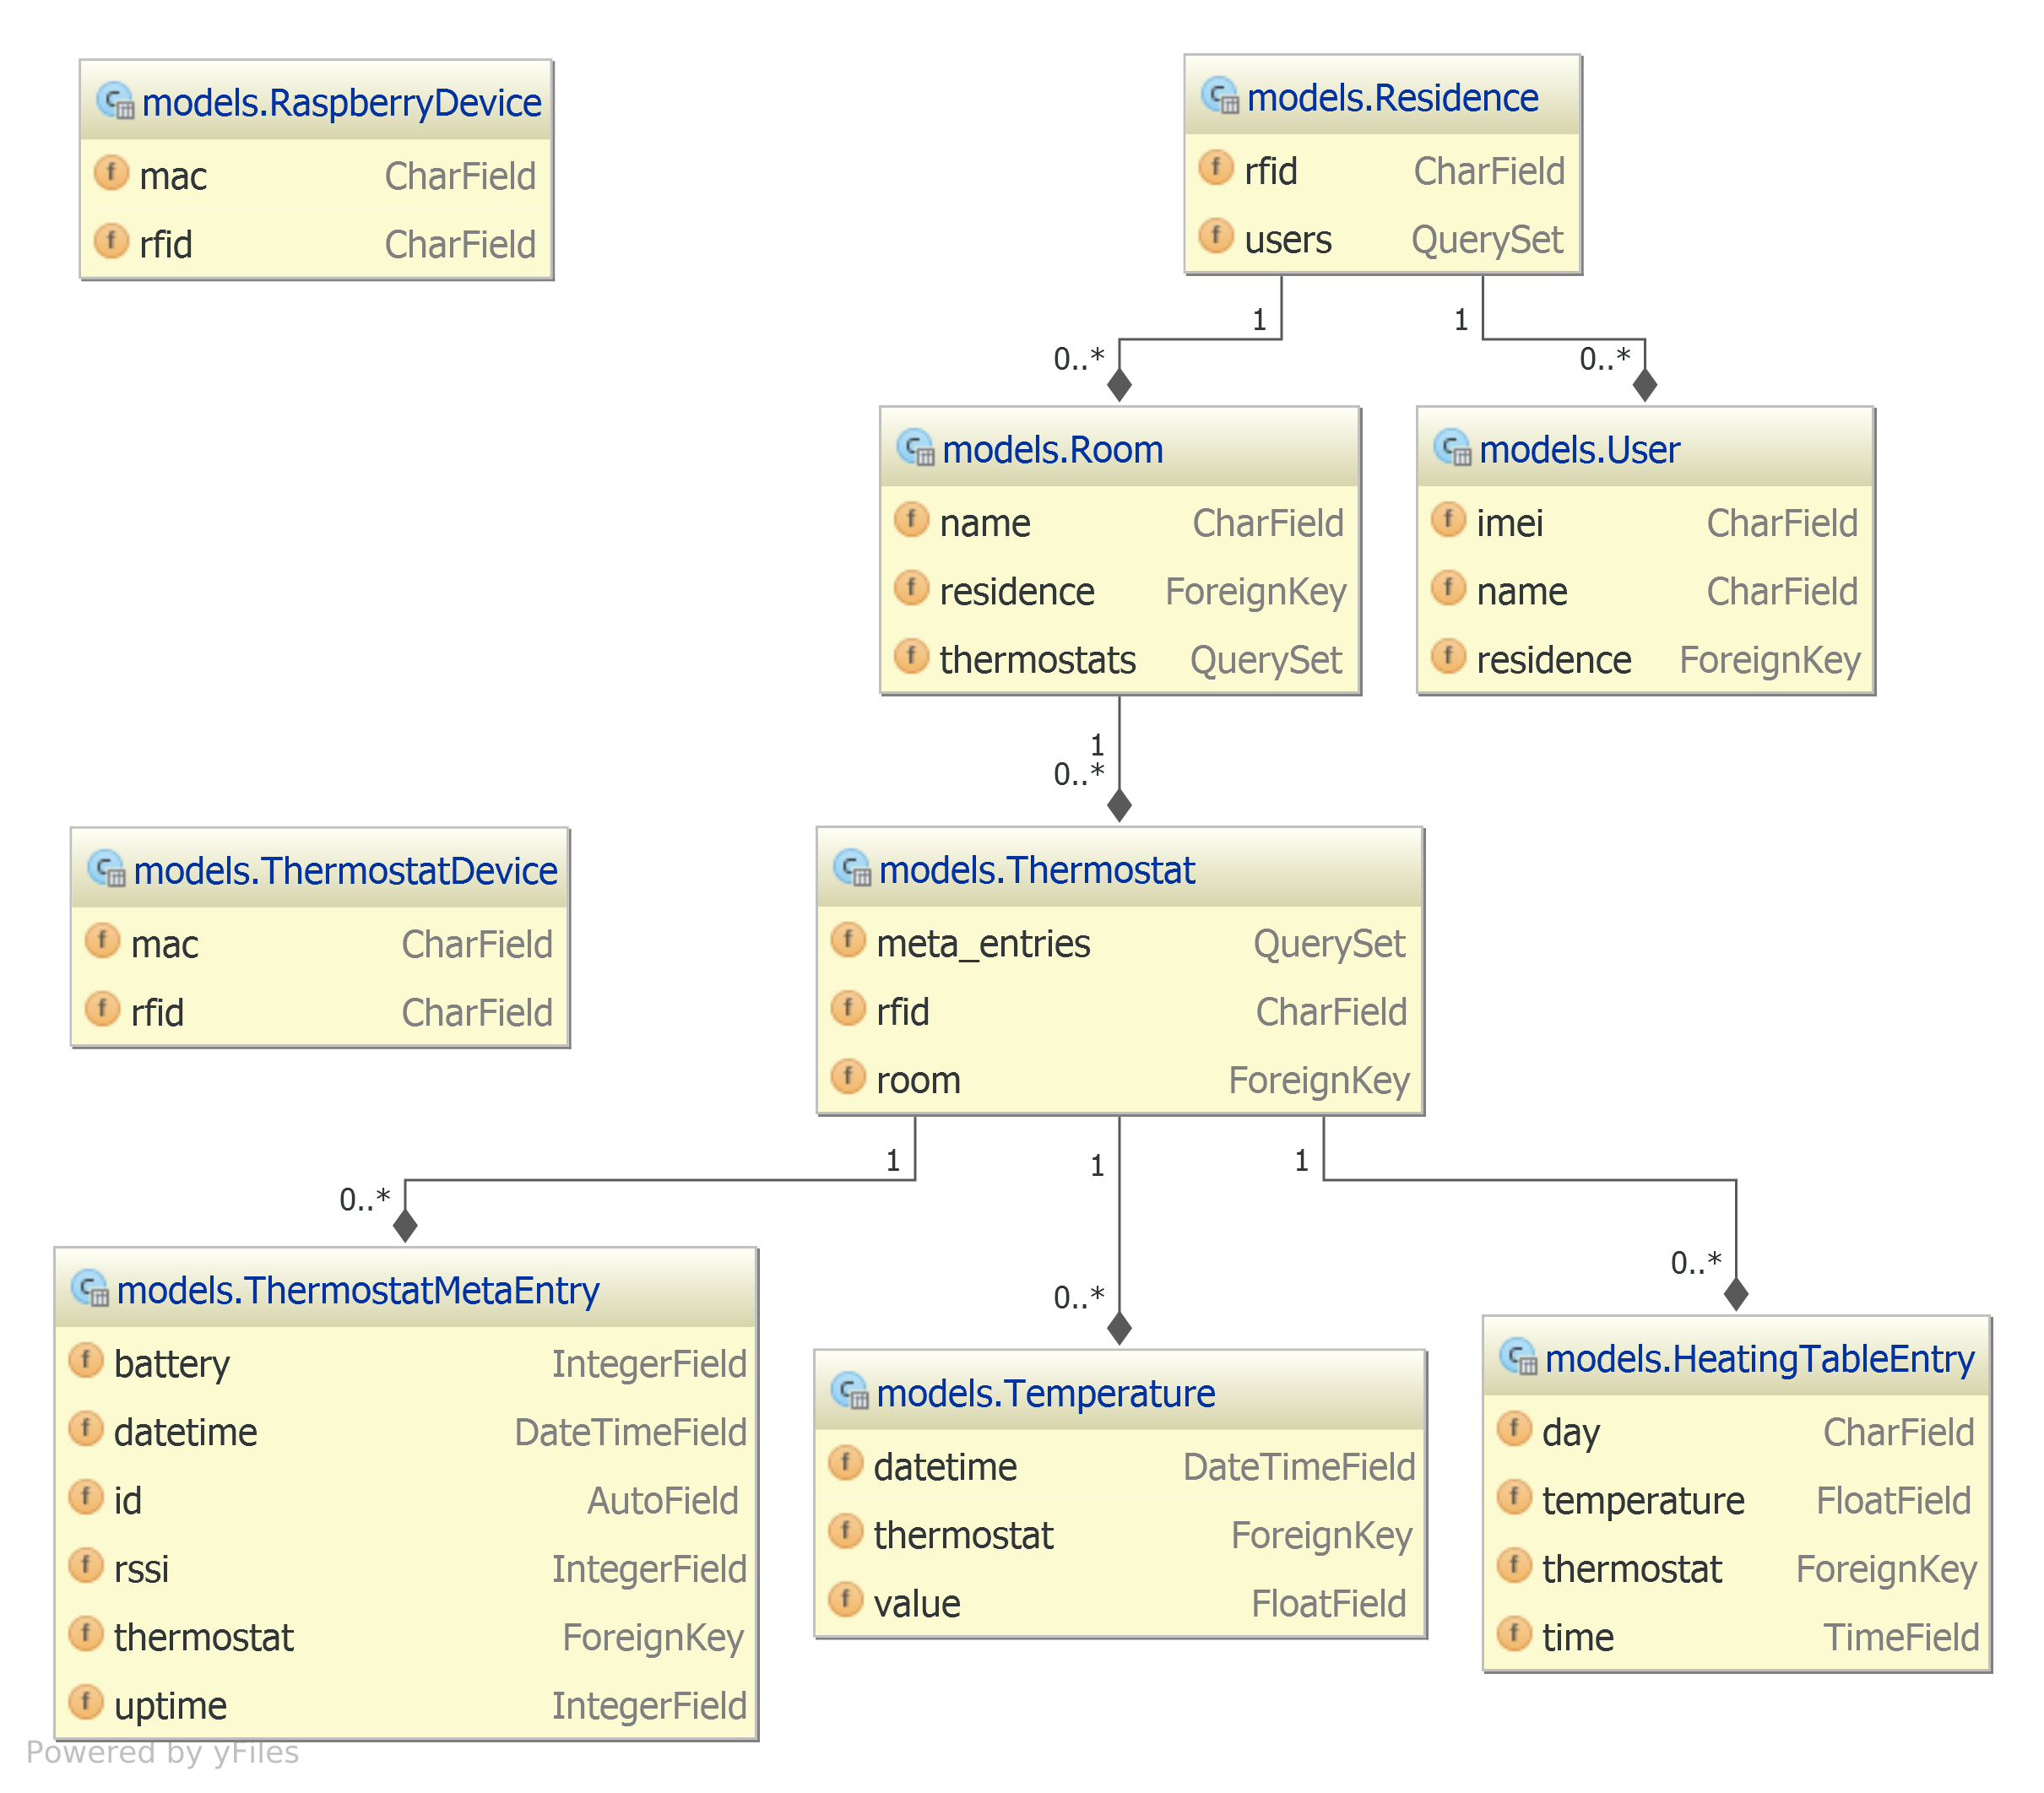
\includegraphics[width=0.8\textwidth]{images/uml_class_diagram_pycharm_highres.png}
\end{center}
\caption{UML class diagram of the models.\todo[inline]{Fix diagram: add all or remove all Querysets. Decide whether or not to display unique constraints.}}
\label{fig:class_diagram}
\end{figure}

Thermostats are organized within rooms and belong to a residence. See Figure~\ref{fig:class_diagram} for a graphical representation of the used models.

\paragraph{Residence}

is identified by the radio frequency identification (RFID) tag number on the deployed local communication gateway. A residence combines users and rooms with their associated thermostats and data into a single encapsulated unit.

\paragraph{User}

is identified by the smart phone's serial number\footnote{The International Mobile Equipment Identity (IMEI), a 15-digit serial number associated to each cell phone, is used to identify each user} and can be registered to at most one residence. 

Room, Thermostat, Temperature, Heating Table Entry, Meta Entry

% temperatures and other data from the local deployment as also the heating schedule from the mobile app.



\subsubsection{Serializers}

\subsubsection{Views}

\subsubsection{Routers}



\subsection{Automated Testing}

Automated software testing is an important part of this project. Django and also the Django REST Framework facilitate automatic testing by providing several classes and tools helping to write and execute tests. Automatic software testing allows the application of test-driven development practices to ensure high software quality.

Furthermore the usage of an Continuous Integration service like Travis CI\footnote{\url{https://travis-ci.org/}} ensures the periodic execution of all tests and logging of the test results.

\subsubsection{Practically Oriented Documentation}

\todo{Screenshot of github.com/spiegelm/smart-heating-server}

\section{Local Deployment}
\label{sec:local_infrastructure}

The local deployments consists of the residential communication gateway and the deployed thermostats with their wireless adapters. The communication gateway collects the data read from the thermostats and sends it to a remote web server. The thermostats are programmable and allow us to modify their behaviour by replacing and adapting the flashed firmware. This project uses the work of previous lab projects as a basis to build upon. The primary focus is to improve the basic functionality of the communication gateway and create an unified but loosely coupled infrastructure by using the RESTful API provided by the server.
See also Figure~\ref{fig:residence_layout} for an overview of the local deployment.

\begin{figure}[h]
\begin{center}
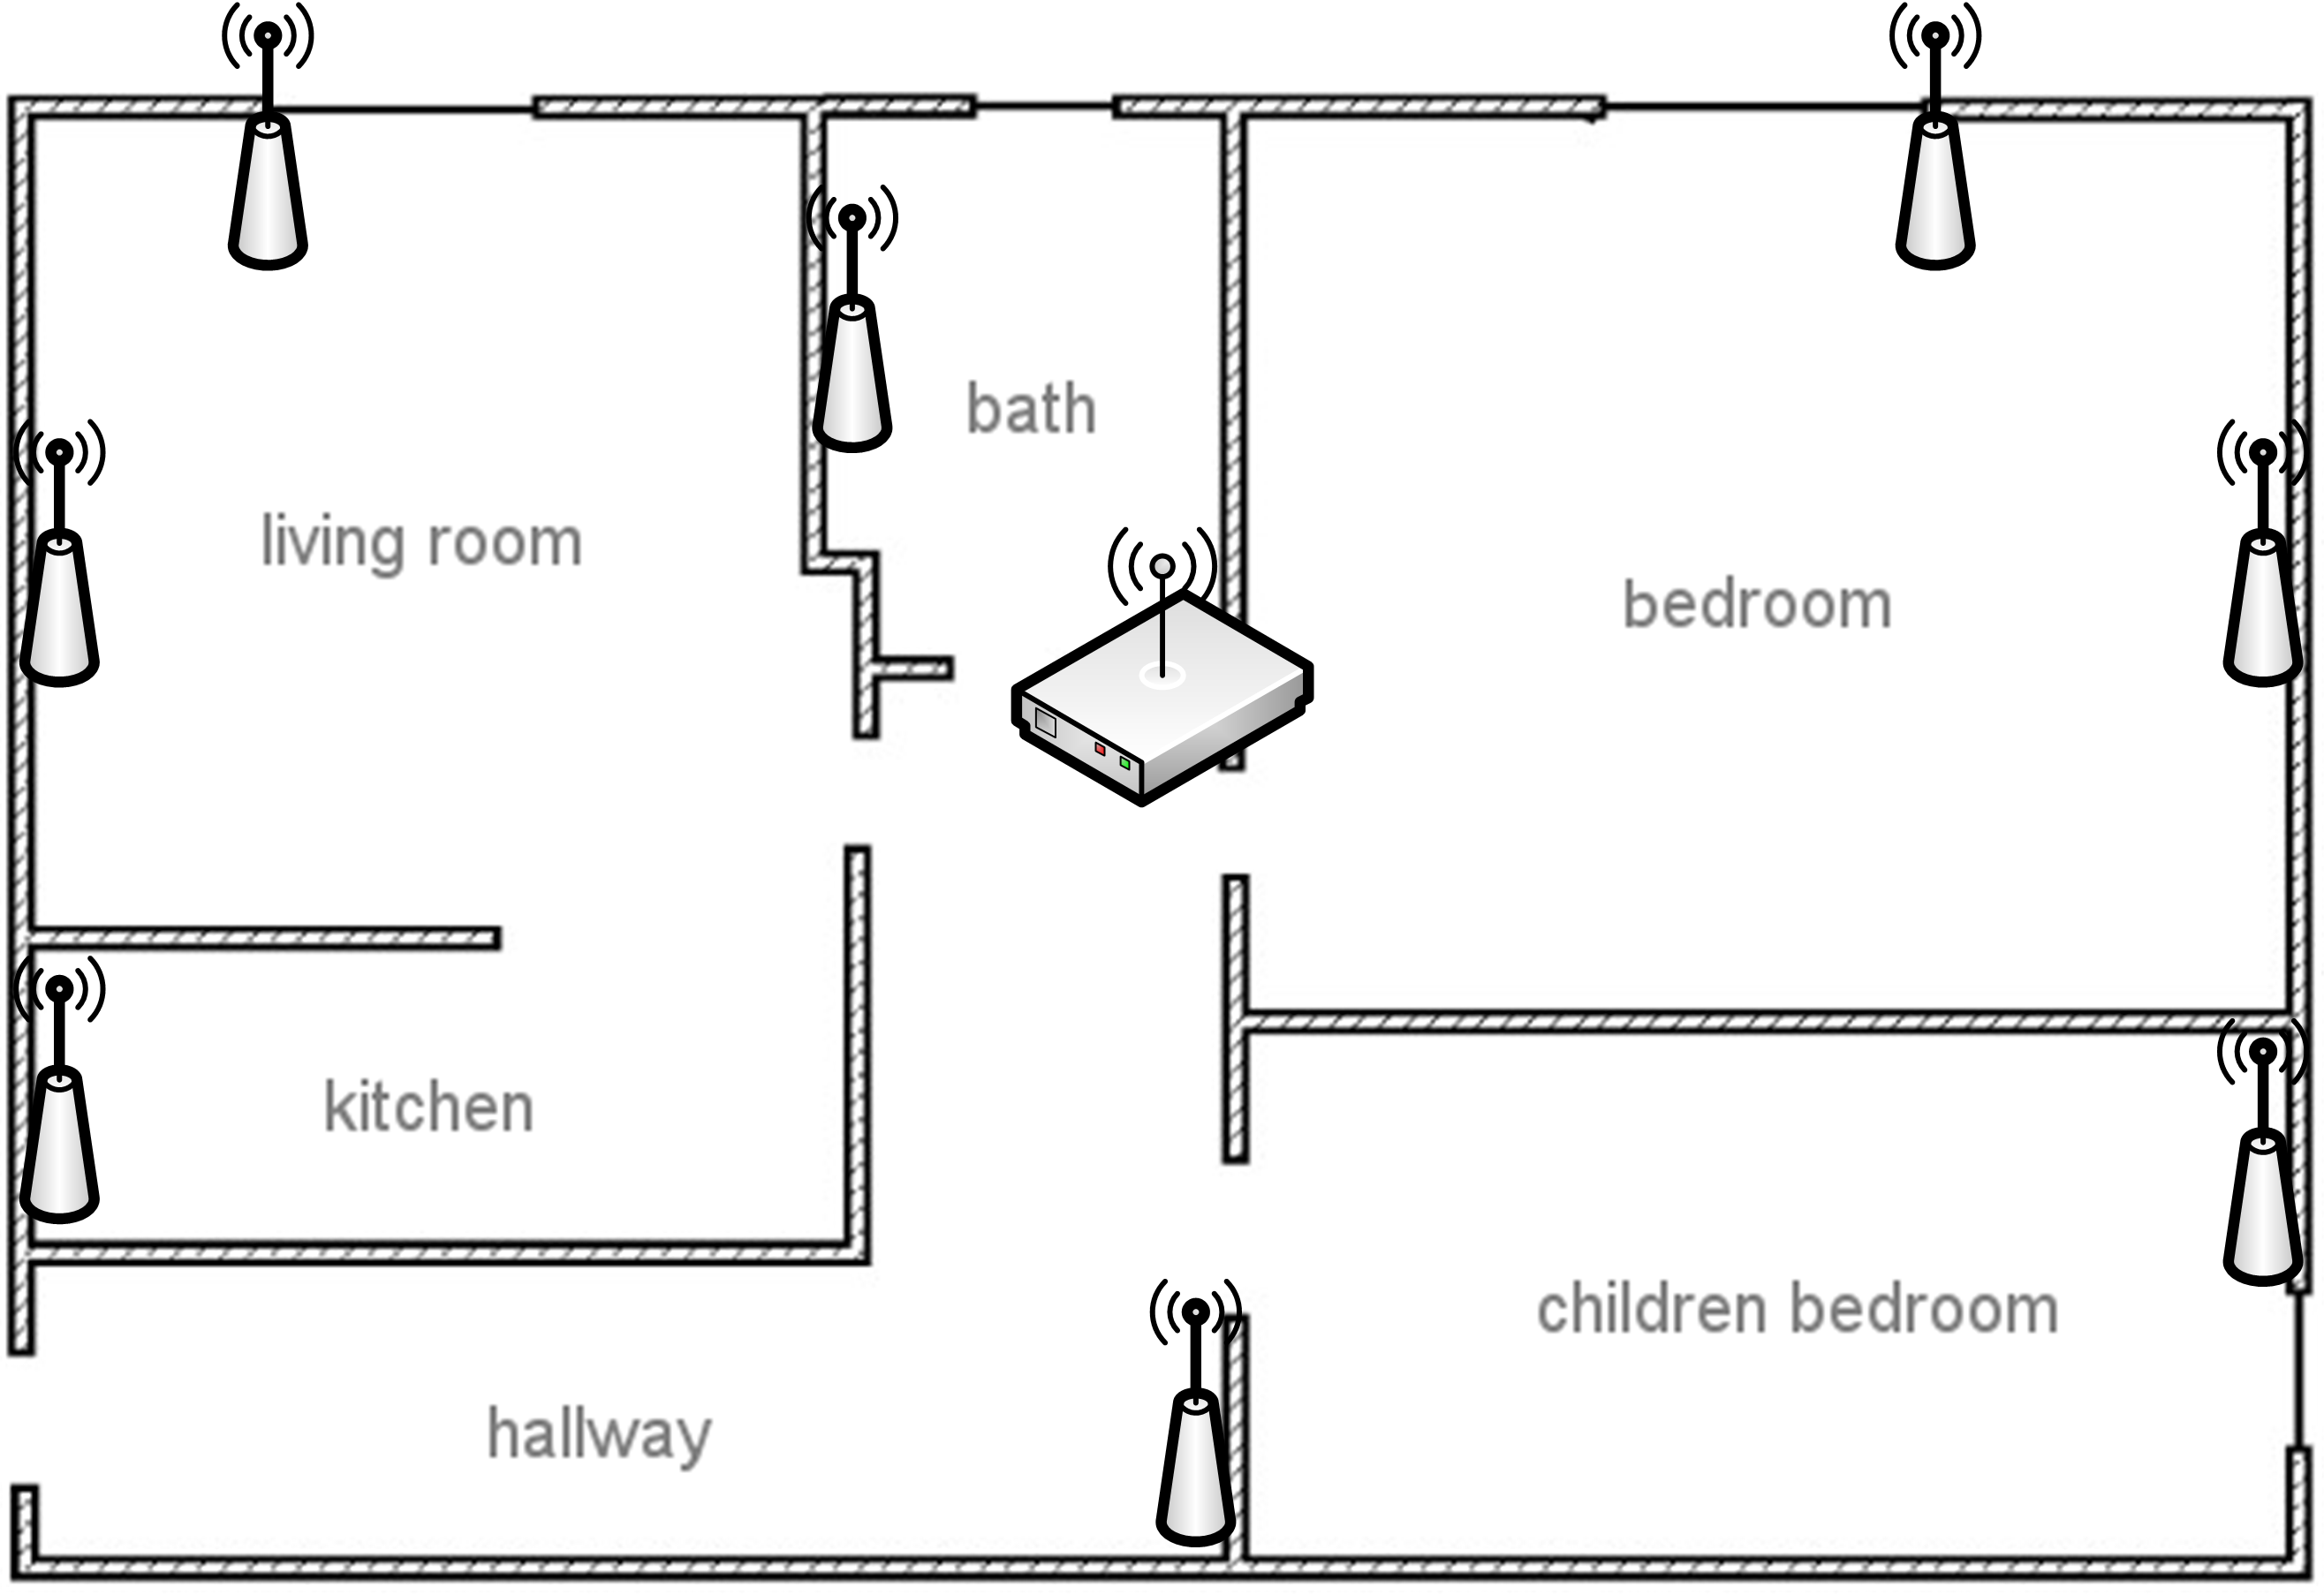
\includegraphics[width=0.8\textwidth]{images/residence_layout_schema.png}
\end{center}
\caption{Example of a residence layout depicting a possible deployment. The local communication gateway is installed in the hallway, connected to the internet and has wireless connections to the deployed thermostats represented as antennas. Source of the original image: \url{http://www.haus-topplicht.de/wp-content/uploads/2013/12/planwohnung2.jpg}}
\label{fig:residence_layout}
\end{figure}

\subsection{Existing Infrastructure}

This lab project builds upon work previously done at the Distributed System Group\footnote{\url{https://www.vs.inf.ethz.ch/}}. 

\subsubsection*{Hardware}

Thermostats, etc

\subsubsection*{Software}

Willis Scripts

\subsection{Design Goals}

Simple, Reliable, Failure resistant

\subsection{Platform and Frameworks}

tunslip6, Python, COAP, aiocoap, requests

\subsection{Implementation}

The communication gateway collects, caches and processes the data read from the thermostats as also the control commands from the server. The local communication gateway works as a proxy server and enables the local deployment to operate independently from the connection to the remote server. This way the last downloaded heating schedule is kept and operated until the server connection is be reestablished. 
%Die grundlegende Einheit jedes Deployments ist die Residence. Eine Residence entspricht genau einem installiertem lokalen System, das die gelesenen Daten der Thermostate sowie Steuerbefehle des Servers sammelt, cached and ausführt. Das lokale Gerät arbeitet als ein lokales Gateway und sorgt dafür, dass der lokale Teil unabhängig von der Verbindung mit dem remote Server funktioniert.
% Temperaturen und andere Meta-Daten von den angebundenen Thermostaten sammelt und cached.


%!TEX root = ../thesis.tex

\section{Server Infrastructure}
\label{sec:server_infrastructure}

The server is the main storage and communication center of this project.
It persists data collected by the local deployment as also organizational information and heating schedules provided by the user via the Mobile App.

\subsection{Design Goals}

\begin{itemize}
\item \emph{Modularity} for independent, interchangeable components for improved Maintainability.
\item \emph{Extensibility} to easily add new resources and relationships.
\item \emph{Usability} for developers.
\item \emph{Testability} for good and comprehensible tests.
\end{itemize}

\subsection{Platform and Frameworks}

The server is implemented with Python, a general-purpose, multi-paradigm programming language\footnote{\url{https://www.python.org/}}.
Python was chosen as it is suitable for developing a solid web server as also for usage on restricted hardware like the Raspberry Pi used for the local deployment.
Django is a popular, open-source web application framework\footnote{\url{https://www.djangoproject.com/}} based on a model-view-controller (MVC) pattern facilitating the development of complex, database-driven web applications.
The Django REST Framework\footnote{\url{http://www.django-rest-framework.org/}} extends Django to support the design of RESTful Web APIs.

\subsection{RESTful API}

The server provides a RESTful\footnote{Note: REST is a programming paradigm where as RESTful is used to describe a web application implementing such an paradigm.} API to access a persistent storage providing the basic CRUD operations: Create, Read, Update and Delete.
Representational State Transfer (REST) is a programming paradigm used in distributed systems especially for machine-to-machine communication.
RESTful web services use HTTP as their preferred communication protocol.

REST is about resources.
Each resource is identified by a uniform resource identifier (URI) and is accessible via the request methods defined in HTTP.
There are two major types of URIs, resource collections and resource representations.
First, a resource representation is a view of its resource's state and is encoded in a transferable format.
This project uses the simple JavaScript Object Notation (JSON) format to represent resources.
Second, resource collections contain representations of the same type of a resource.

\paragraph{Design Decisions}

\begin{enumerate}
    \itemsep0em
    \item The underlying model hierarchy is represented via nested URLs.
    \label{enum:design_decision_nested_urls}
    \item The resource identifier is the first field in each resource representation.
    \item Within resource representations, collections are referenced per URL. Resources are referenced by including their representation.
    \label{enum:design_decision_resource_referencing}
    \item URL fields are identified by the name \highlight{url} or the suffix \highlight{\_url}. Each resource representation contains its own URL in the field \highlight{url}.
    \label{enum:design_decision_url_fields_prefix}
\end{enumerate}

See Listing~\ref{lst:room-json-example} for an example of a resource representation.

\begin{snippet}[language=JavaScript,label={lst:room-json-example},caption={Example representation of the Room resource at \nolinkurl{http://server/residence/04891BB9232584/room/2/}.
		The \highlight{url} field determines the URL of the represented resource.
		Within the \highlight{residence} field the representation of the associated Residence resource is nested.
		The included Residence representation has its own \highlight{url} field.
		Collections of the Residence's Rooms and Users are not nested but referenced via URL to limit the response size.}]
	{
		"id": 2,
		"url": "http://server/residence/04891BB9232584/room/2/",
		"name": "Dining Room",
		"residence": {
			"rfid": "04891BB9232584",
			"url": "http://server/residence/04891BB9232584/",
			"rooms_url": "http://server/residence/04891BB9232584/room/",
			"users_url": "http://server/residence/04891BB9232584/user/"
		},
		"thermostats_url": "http://server/residence/04891BB9232584/room/2/thermostat/"
	}
\end{snippet}


\paragraph{Browsable API}

The Django REST Framework offers the ability to dynamically generate a browsable interface accessible per web browser.
It includes a formatted output of the JSON response, offers forms to add new resources and edit or delete existing resources and displays URLs as clickable hyperlinks.
This interface is an additional HTML output format enabling developers to easily interact with the API without the need of external tools.
The Browsable Web API is designed for readability where as the API renders its data as compressed JSON to reduce transmission bandwidth.
See Figure~\ref{fig:server_infrastructure_browsable_api} for an example.

\begin{figure}[h]
	\begin{center}
		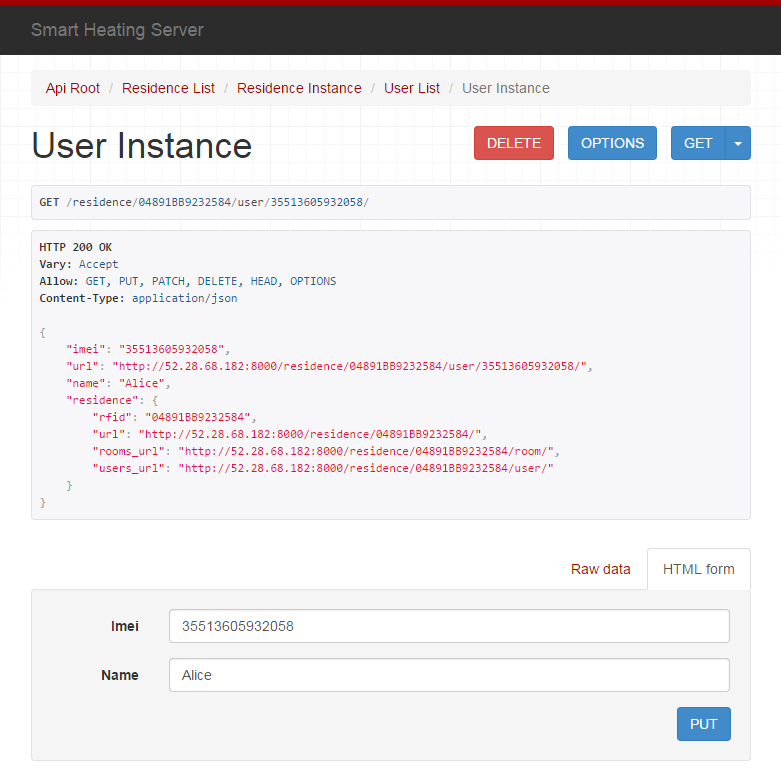
\includegraphics[width=0.8\textwidth]{images/server_browable_api_user_instance.png}
	\end{center}
	\caption{Screenshot of the Browsable Web API showing an instance of an user resource. The interface allows the developer to easily edit or delete the user as well as to navigate the residence or its associated room or user collection.}
	\label{fig:server_infrastructure_browsable_api}
\end{figure}


\subsection{Program Architecture and Implementation}

The server implementation is built on the Django Framework following a variation
%\footnote{For the interested reader: \url{https://docs.djangoproject.com/en/1.8/faq/general/\#django-appears-to-be-a-mvc-framework-but-you-call-the-controller-the-view-and-the-view-the-template-how-come-you-don-t-use-the-standard-names}}
of the Model-View-Controller (MVC) architectural pattern.
We assume the user to be familiar with the common MVC pattern\footnote{We refer the interested reader to \url{https://en.wikipedia.org/wiki/Model-view-controller}}.

\subsubsection{Models}
\label{sec:server_infrastructure_models}

Models structure the underlying data and provide operations for manipulating it.
In Django models contain the business logic and are also responsible for validating user input and providing appropriate error messages.
The \highlight{smart\_heating.models} namespace contains all project models.
Each model extends the abstract \highlight{Model} class providing a general method used to get an objects representation for debugging purposes as well as the abstract \highlight{get\_recursive\_pks} method.
The later method is used to generate hierarchical URLs and will be further described in Section~\ref{sec:server_infrastructure_serializers}
% A high level description of all used models is given in Section~\ref{sec:system_overview_models}. 

\begin{figure}[h]
\begin{center}
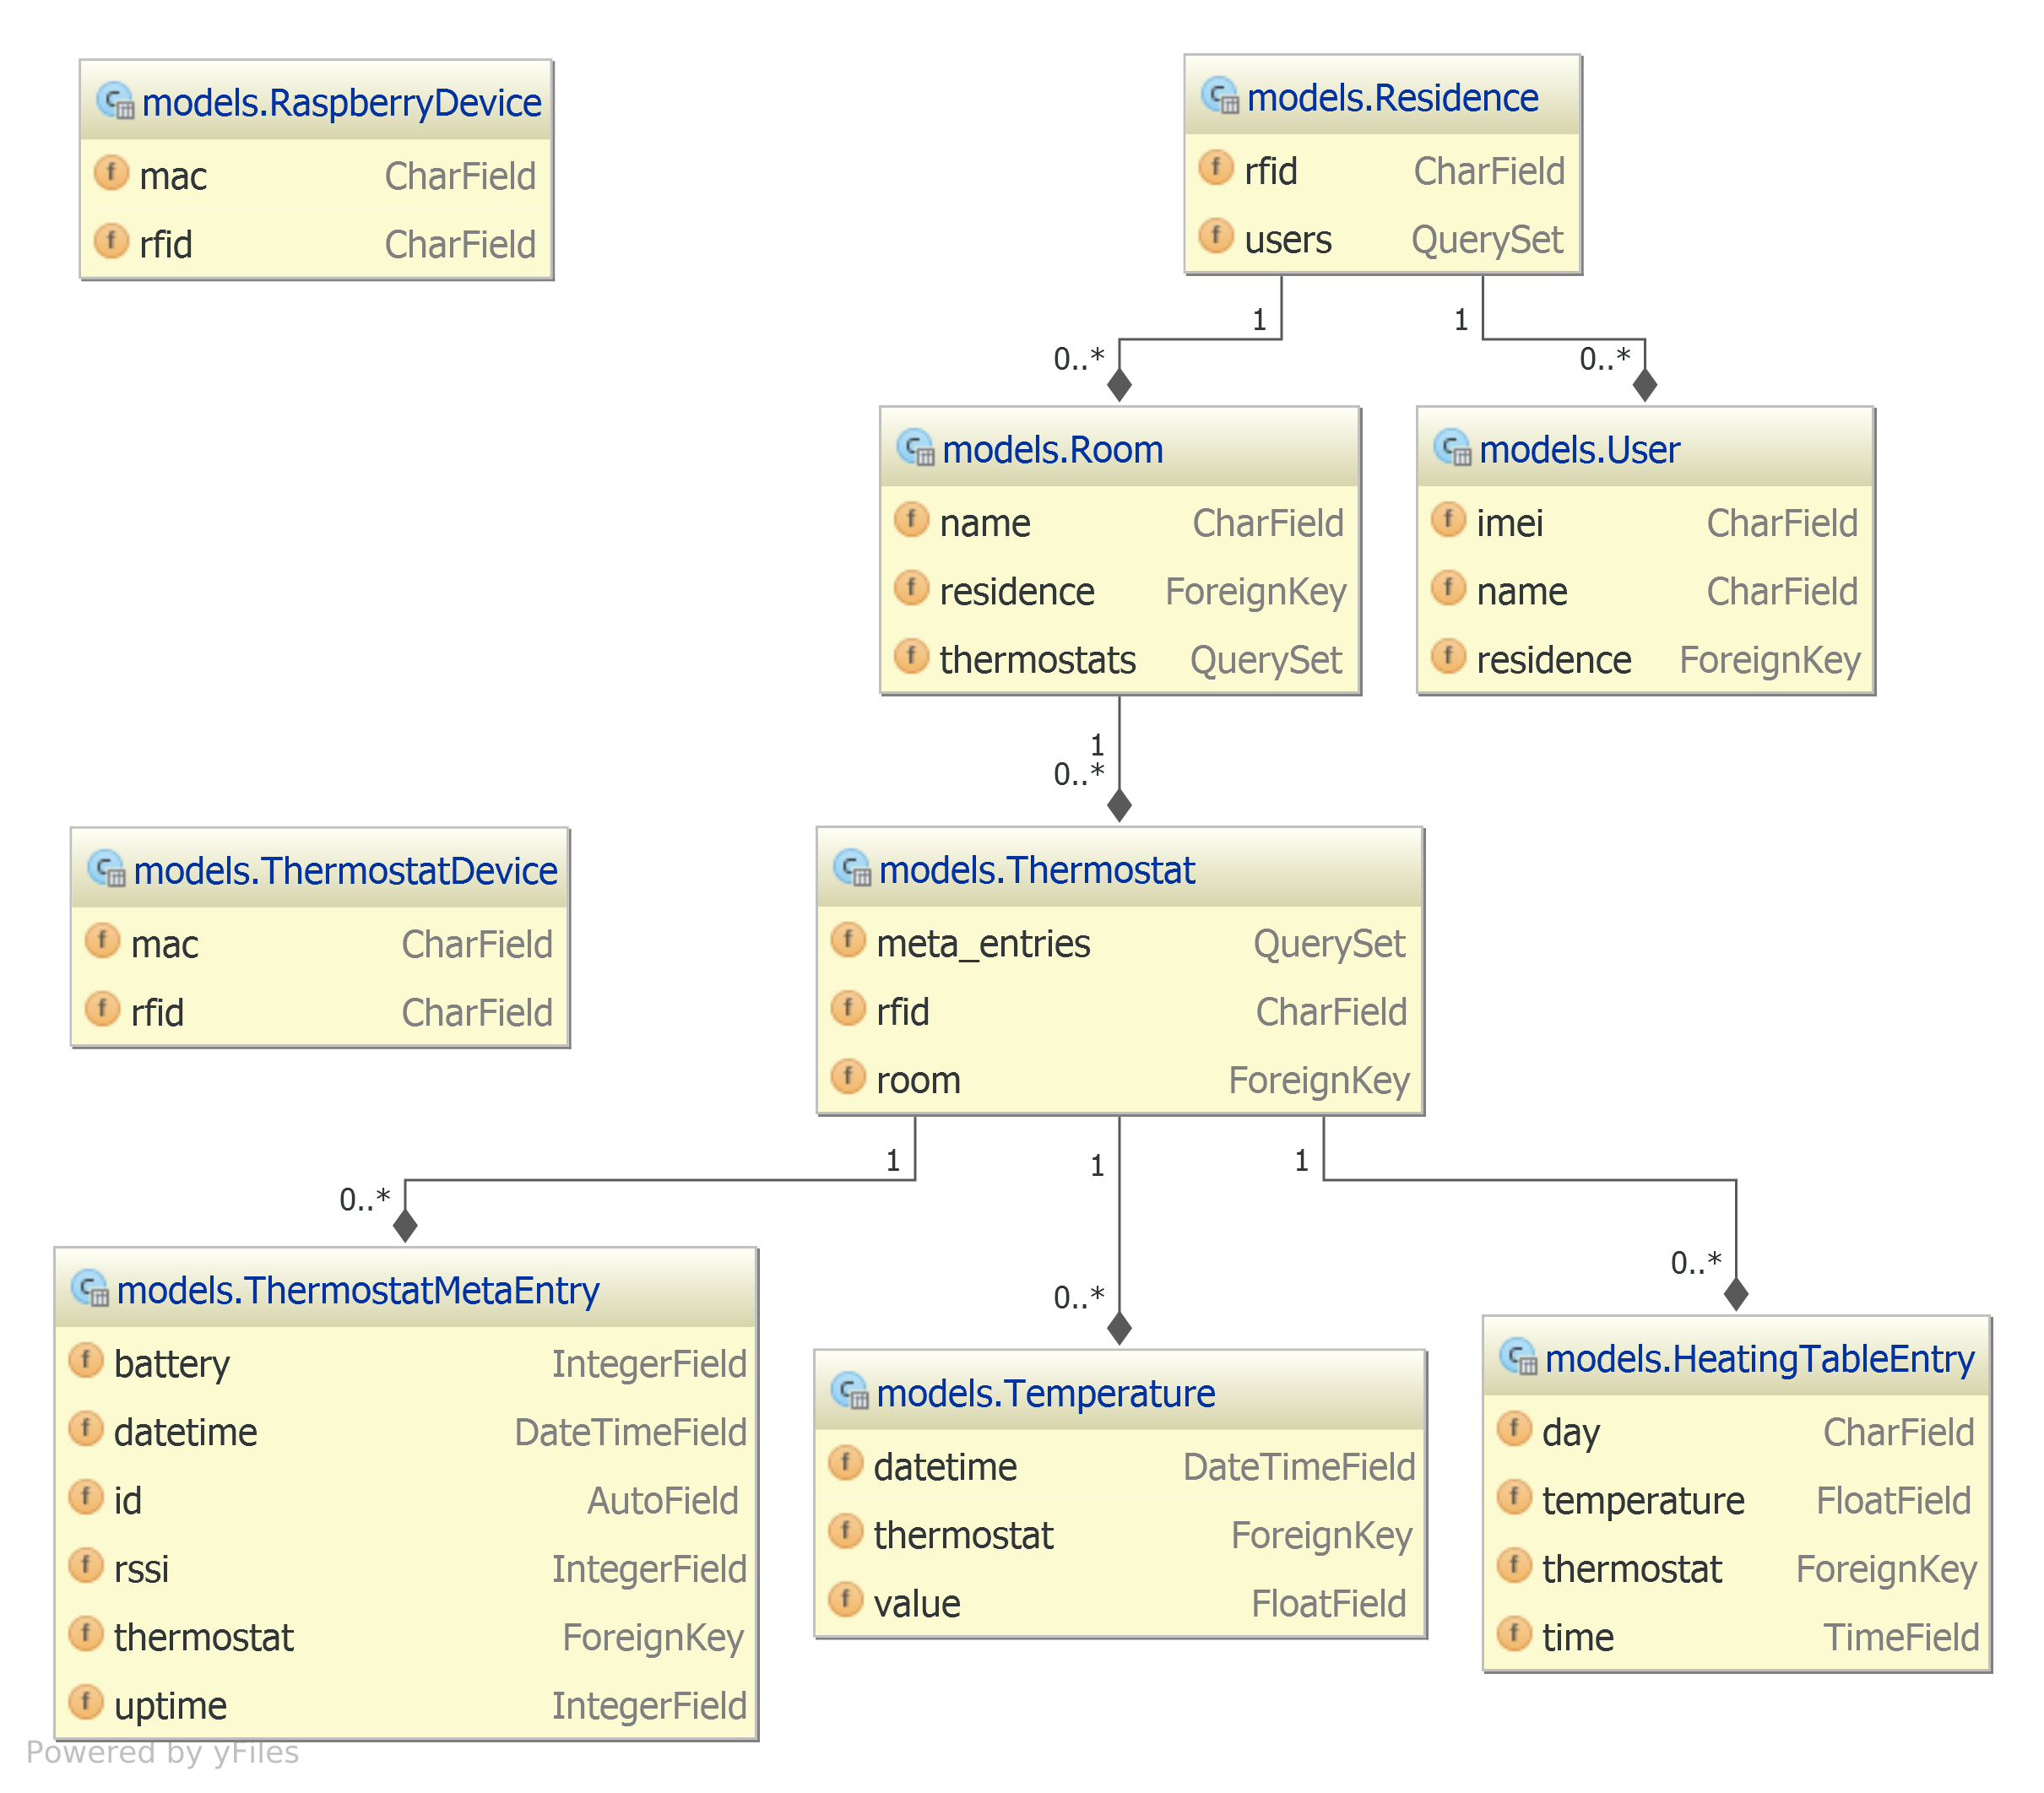
\includegraphics[width=0.8\textwidth]{images/uml_class_diagram_pycharm_highres.png}
\end{center}
\caption{UML class diagram of the models.\todo[inline]{Fix diagram: add all or remove all Querysets. Decide whether or not to display unique constraints.}}
\label{fig:class_diagram}
\end{figure}

Thermostats are organized within rooms and belong to a residence. See Figure~\ref{fig:class_diagram} for a graphical representation of the used models.

\paragraph{Residence}

is identified by the radio frequency identification (RFID) tag number on the deployed local communication gateway. A residence combines users and rooms with their associated thermostats and data into a single encapsulated unit.

\paragraph{User}

is identified by the smart phone's serial number\footnote{The International Mobile Equipment Identity (IMEI) is a 15-digit serial number associated to each GSM cell phone.} and can be registered to at most one residence.

Room, Thermostat, Temperature, Heating Table Entry, Meta Entry
\todo[inline]{Finish models}

% temperatures and other data from the local deployment as also the heating schedule from the mobile app.

\subsubsection{Serializers}
\label{sec:server_infrastructure_serializers}

Serializers are responsible for translating models into a transmittable format and reverse.
This project uses JSON as the transmittable format.
Each model has an associated serializer which determines which model fields should be included into the resource representation.
Additional fields can be added to the representation or individual field representations can be overwritten to offer customized output.

A commonly used customization is the replacement of the default \highlight{HyperlinkedIdentityField} with \highlight{HierarchicalHyperlinkedIdentityField}.
This custom serializer field generates URLs according to the hierarchical schema applied in this project.
For example the URL for a room would be \nolinkurl{http://server.com/residence/041FB2B9232580/room/5/}.
To assemble this URL not only the identifier of the room but also the identifier of its parent are required.
The adapted field extends the default field and provides all identifiers of the hierarchy required to generate the URL by using the hierarchical base class \highlight{smart\_heating.models.Model}.

Nested resources are implemented using nested serializers.
This way existing serializers can be reused to include their resource representation into another representation.
% \item Within resource representations, collections are referenced per URL. Resources are referenced by including their representation.


\subsubsection{Views}
\label{sec:server_infrastructure_views}

A view is a class which processes requests and returns a response.
Django defines the view as the place that defines how but also which data is presented.
This slightly differs from the traditional MVC architectural pattern but will not be explained in detail here\footnote{For more details we refer the reader to \url{https://docs.djangoproject.com/en/1.8/faq/general/\#django-appears-to-be-a-mvc-framework-but-you-call-the-controller-the-view-and-the-view-the-template-how-come-you-don-t-use-the-standard-names}}.
Django includes generic view classes and mixins to provide common functionality and to facilitate code reuse.
The Django REST Framework further abstracts views by supplying \highlight{ViewSets}.
These \highlight{ViewSets} facilitate the unified handling of different HTTP methods within a single class for each public resource.

The used \highlight{ModelViewSet} is such a class serving as a base for individual view sets of a resource.
In the simplest case only requires the definition of a database query and an appropriate serializer class.
The \highlight{ResidenceViewSet} is a good example of a view class consisting of only 3 lines of code.

\paragraph{Pagination} is the practice of partitioning lists into smaller pieces.
In this project pagination is used for expectedly large resource collections such as temperatures or meta entries.
The applied pagination style depends on two parameters: \highlight{limit} and \highlight{offset}.
Limit determines the page size, i.e. the maximum number of items that are displayed simultaneously.
Offset determines the starting item.\\
The custom pagination class \highlight{pagination.BasePagination} implements the design decision \ref{enum:design_decision_url_fields_prefix} to suffix resource field names representing links.

\subsubsection{Routes}
\label{sec:server_infrastructure_routers}

URLs are defined explicitly in the file \highlight{smart-heating/urls.py}.
For each request the responsible view is determined by matching the requested URL against a list of regular expressions.
This technique allows flexible configurations as required for the hierarchical URL scheme.


\subsection{Automated Testing}

Automated software testing is an important part of this project. Django and also the Django REST Framework facilitate automatic testing by providing base classes and tools helping to create and execute tests.

The tests are designed to infer the functionality and behavior of the application.
An executed test run shows at any particular time which functional requirements are fulfilled and which are not.
Look at Listing~\ref{lst:test_report} for an example.
These dynamically generated test reports nicely complement traditional documentation and also provide small informational code examples that are shown to work.
%Die Tests sind so designed, dass sie Rückschlüsse auf die Funktionalität der Applikation geben. Ein ausgeführter Test-Run zeigt welche funktionalen Anforderungen erfüllt sind und welche nicht.
During application development we intensively used test driven development practices to increase productivity and achieve high software quality.
Automatic software testing allows to already formulate the requirements of a computer program such that they can be automatically checked before and during application development.
%Während der Applikationsentwicklung wurde intensiver Gebrauch von Test-getriebenen Entwicklungspraktiken gemacht, um die Produktivität und Softwarequalität zu steigern. Automatisiertes software testing ermöglicht es Anforderungen an ein Computer Programm bereits im vorhinein so zu formulieren, dass sie schon während der Implementierung automatisiert überprüft werden können.
%Automatic software testing allows the application of test-driven development practices to ensure high software quality.

\begin{snippet}[label={lst:test_report},caption={Excerpt of the test output with verbosity level 2 documenting the application behavior},numbers=none]
$ python manage.py test -v 2
	[...]
	smart_heating.tests.test_api.ViewRootTestCase
		test_root_contains_residence_url ... ok
	smart_heating.tests.test_api.HeatingTableTestCase
		test_create_heating_table_entry ... ok
		test_heating_table_entries_are_ordered_by_date_and_time ... ok
		test_heating_table_entry_representation ... ok
		[...]
	smart_heating.tests.test_api.ViewUserTestCase
		test_create_user ... ok
		test_get_non_existent_imei_is_404 ... ok
		test_get_user_of_unrelated_residence_is_404 ... ok
		test_user_collection_contains_user_representations ... ok
		test_user_representation_contains_imei_and_name ... ok
		[...]
-------------------------------------------------------------------
Ran 58 tests in 0.765s
OK
\end{snippet}


Furthermore the usage of an Continuous Integration service like Travis CI\footnote{\url{https://travis-ci.org/}} ensures that individual development branches are consistently tested and don't break the main development line upon branch integration.
Additionally this convenient services ensures the periodic execution of all tests and logging of the test results.

%!TEX root = ../thesis.tex

\section{Local Deployment}
\label{sec:local_infrastructure}

The local deployments consists of the residential communication gateway and the deployed thermostats with their wireless adapters. The communication gateway collects the data read from the thermostats and sends it to a remote web server. The thermostats are programmable and allow us to modify their behaviour by replacing and adapting the flashed firmware. This project uses the work of previous lab projects as a basis to build upon. The primary focus is to improve the basic functionality of the communication gateway and create an unified but loosely coupled infrastructure by using the RESTful API provided by the server.
See also Figure~\ref{fig:residence_layout} for an overview of the local deployment.

\begin{figure}[h]
\begin{center}
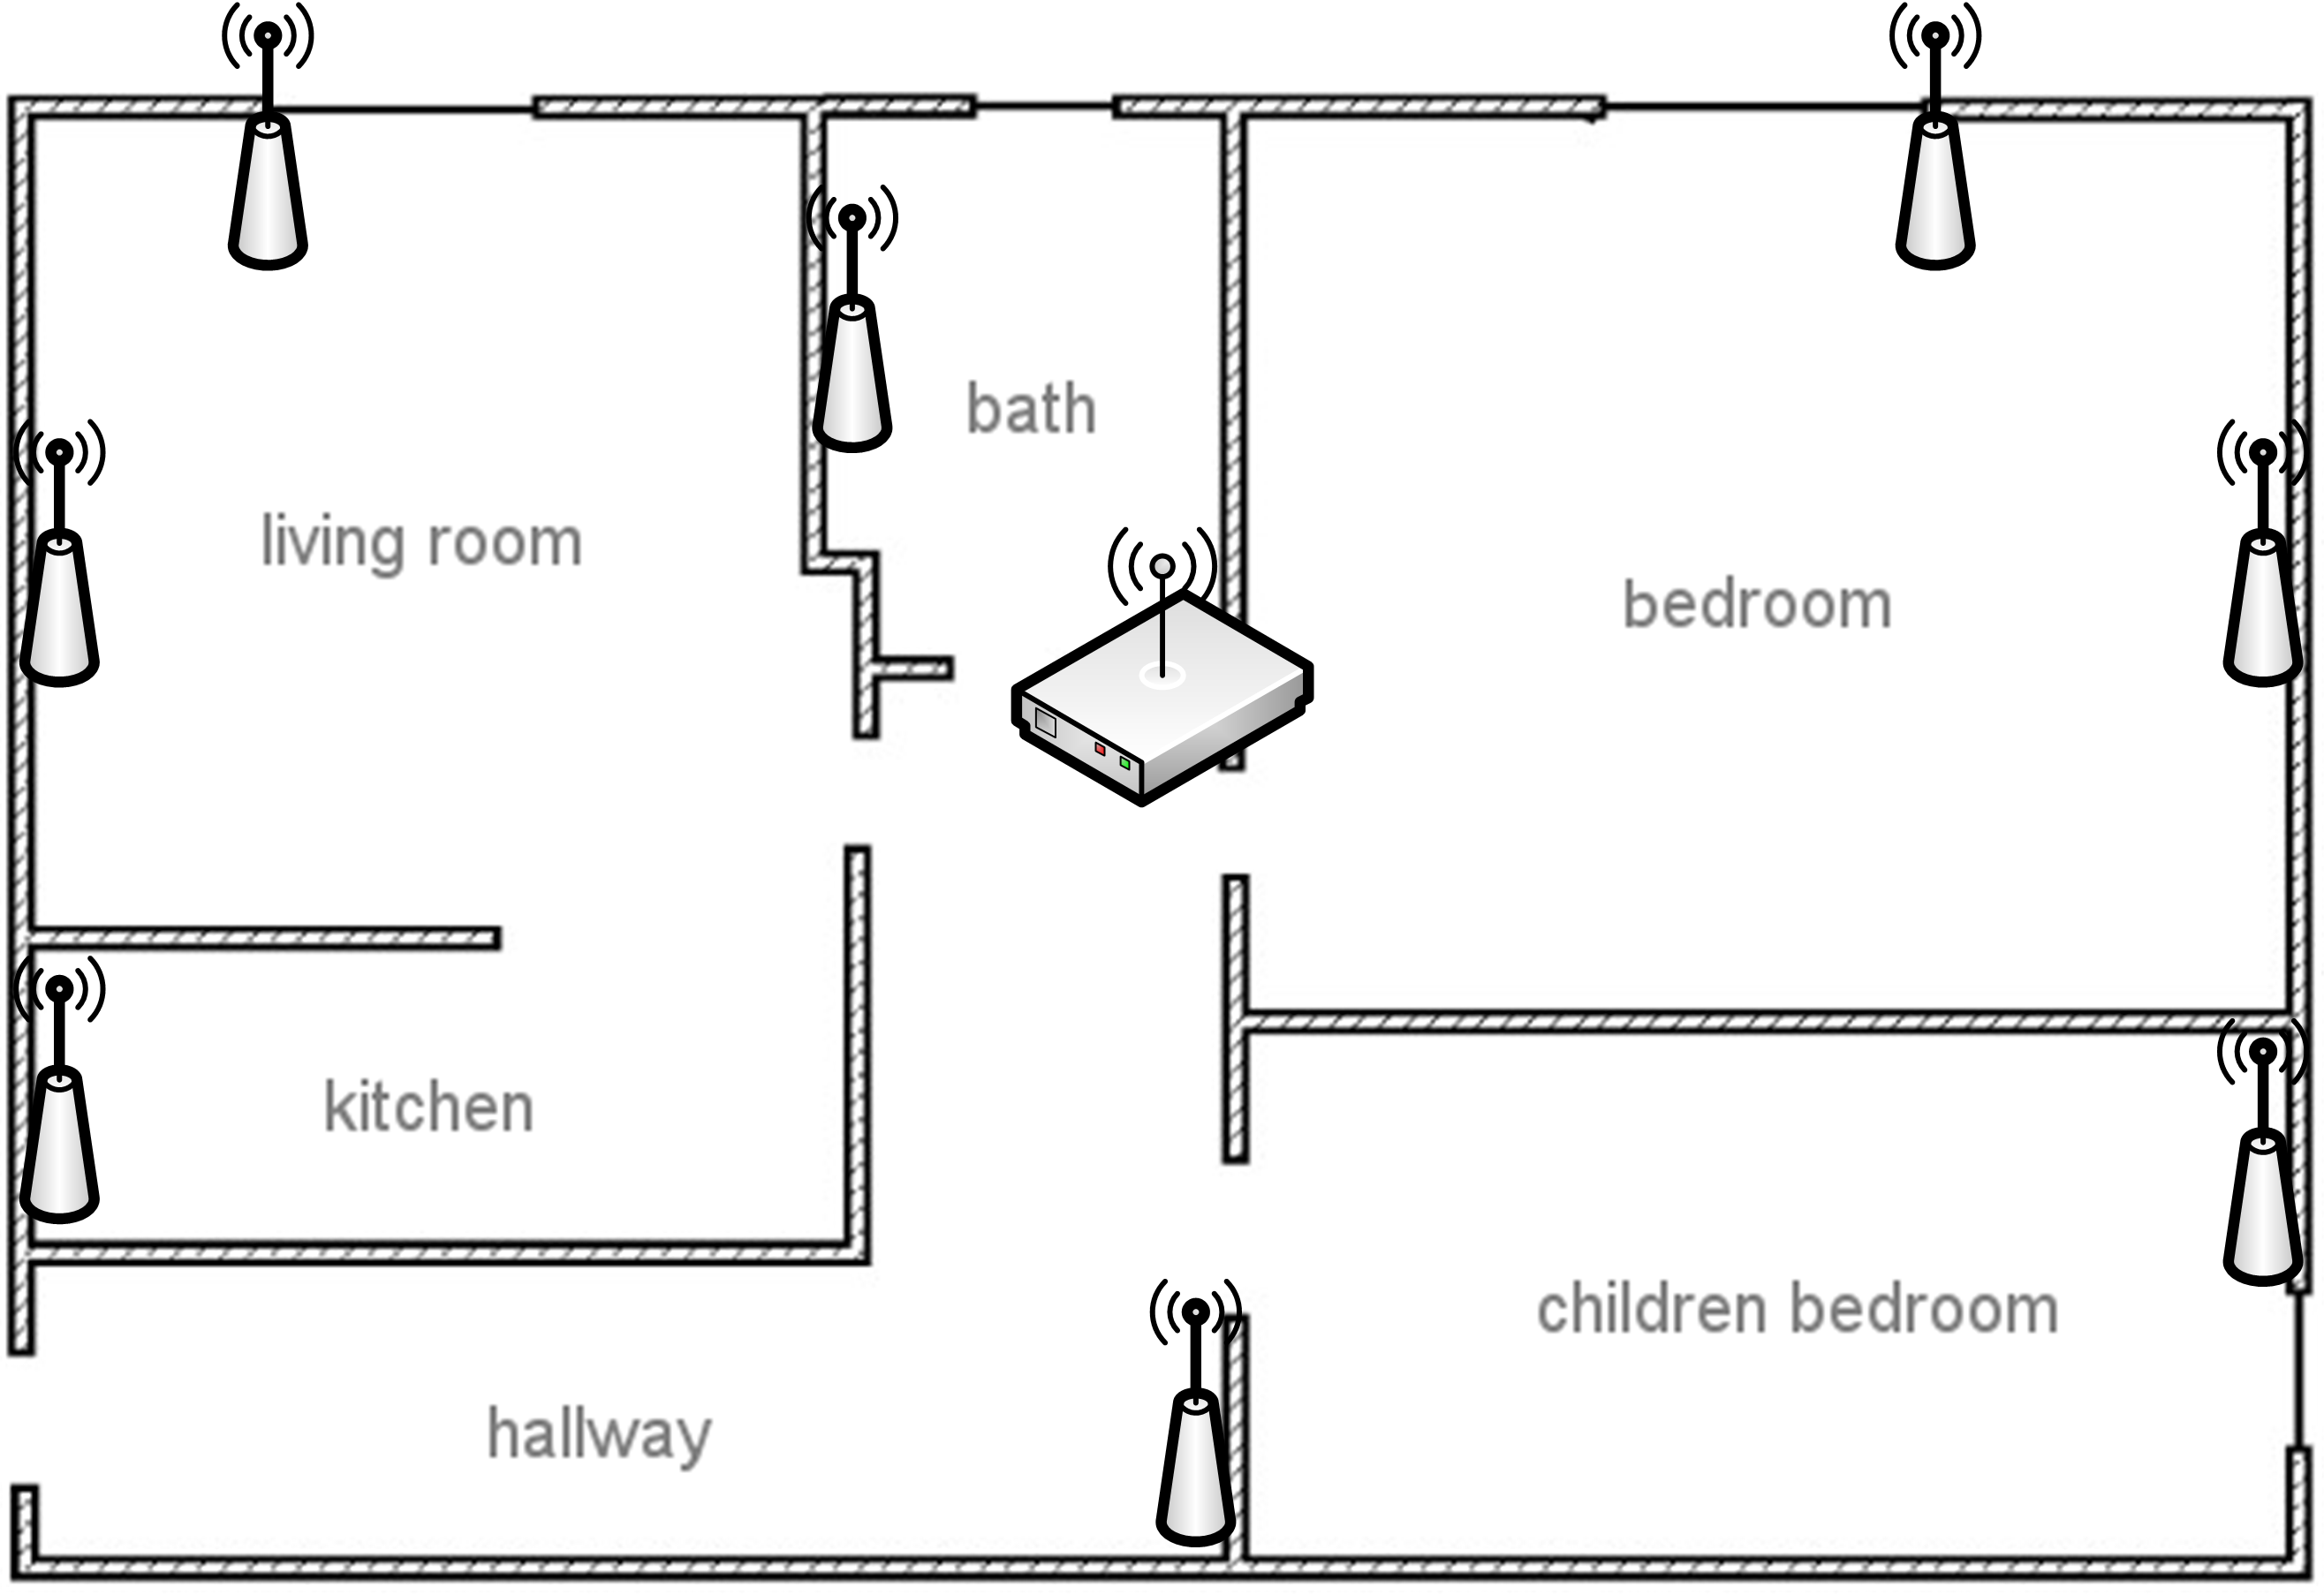
\includegraphics[width=0.8\textwidth]{images/residence_layout_schema.png}
\end{center}
\caption{Example of a residence layout depicting a possible deployment. The local communication gateway is installed in the hallway, connected to the internet and has wireless connections to the deployed thermostats represented as antennas. Source of the original image: \url{http://www.haus-topplicht.de/wp-content/uploads/2013/12/planwohnung2.jpg}}
\label{fig:residence_layout}
\end{figure}

\subsection{Existing Infrastructure}

This lab project builds upon work previously done at the Distributed System Group\footnote{\url{https://www.vs.inf.ethz.ch/}}. 

\subsubsection*{Hardware}

Thermostats, etc

\subsubsection*{Software}

Willis Scripts

\subsection{Design Goals}

Simple, Reliable, Failure resistant

\subsection{Platform and Frameworks}

tunslip6, Python, COAP, aiocoap, requests

\subsection{Implementation}

The communication gateway collects, caches and processes the data read from the thermostats as also the control commands from the server. The local communication gateway works as a proxy server and enables the local deployment to operate independently from the connection to the remote server. This way the last downloaded heating schedule is kept and operated until the server connection is be reestablished. 
%Die grundlegende Einheit jedes Deployments ist die Residence. Eine Residence entspricht genau einem installiertem lokalen System, das die gelesenen Daten der Thermostate sowie Steuerbefehle des Servers sammelt, cached and ausführt. Das lokale Gerät arbeitet als ein lokales Gateway und sorgt dafür, dass der lokale Teil unabhängig von der Verbindung mit dem remote Server funktioniert.
% Temperaturen und andere Meta-Daten von den angebundenen Thermostaten sammelt und cached.


% Define block styles
\tikzstyle{block} = [rectangle, draw, fill=blue!20, 
    text width=5em, text centered, rounded corners, minimum height=4em, node distance=4cm]
\tikzstyle{line} = [draw, -latex']

\chapter{Mobile App}
\label{sec:mobile_app}

Smart heating systems are on the rise. More and more companies are trying to secure a spot in the market offering a variety of features in their control applications, which are mostly mobile or tablet based or even come with their own device. In this section we discuss the Android application we designed and implemented for users to control our heating system. We focused on keeping things simple because as we were researching some of the already existing systems we realized very quickly that the main issue is usability. In almost all cases the user is presented with an abundance of features and extras. Even though most of them would be very useful and effective, the average user will most likely be overwhelmed. Many user interfaces put functionality first. This often results in cluttered designs. Figure \ref{fig:smart_heating_apps} shows some of the user interfaces for controlling smart heating systems. 

In Section \ref{sec:use_cases} we look at some use cases for such control systems and talk about how a general control application would handle them. Afterwards we show our own design of the application for control the smart heating system we are presenting.

Because of the lack of easy to use controlling in already existing systems we chose to focus our design decisions on these aspects. The user is confronted only with a small number of screens which are all visually designed in a way so the user will always immediately know what he is looking at. The different screens are discussed in further detail in Sections \ref{sec:first_view} through \ref{sec:last_view}.

Finally we evaluate our design decisions, reflecting on the use cases to see which ones were covered by our application and which ones were not. Naturally during development we came up with a lot of new ideas for new features and extras for our own application but we decided to stick with the initial design choices to keep it as simple as possible. We will talk more about these ideas in Section \ref{sec:futurework}, where possible future work on this project is listed.

\begin{figure}
	\begin{center}
		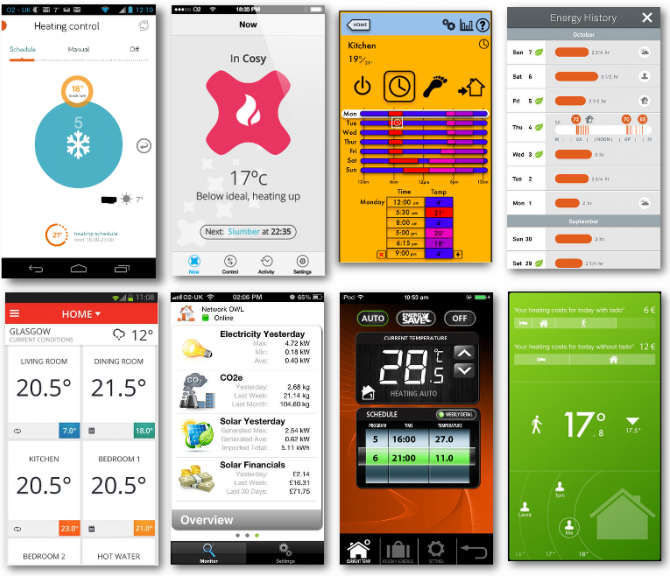
\includegraphics[width=0.8\textwidth]{images/smart_heating_apps.png}
	\end{center}
	\caption{Some examples of mobile applications for controlling smart heatings systems. Source: \url{https://cdn.recombu.com/media/digital/news/legacy/M13058/1397569835_w670_h576.png}}
	\label{fig:smart_heating_apps}
\end{figure}


\section{Use Cases}
\label{sec:use_cases}

We analyze different use cases that an average user might run into while using a smart heating system. This way we are able to ensure that our design decision leads to a simple yet effective application which helps the user control the system in an easy way without overcomplicating things. There is a tradeoff that certain functionality is lost because of these decisions but our main focus was to create an application which is easy to use. 

\begin{enumerate}
\item \textbf{Use Case: User wants to install the system}

Anna has just purchased the smart heating system in the store. After she comes home, she unwraps the components and wants to install the system. The manual tells her to install the mobile app to set up the system. The app guides her through the installation process and allows her to connect the thermostats she manually installed on the radiators to the system.
\item \textbf{Use Case: User feels cold}

Bob is sitting in the living room feeling cold. He starts the mobile app to access the temperature settings for the living room. He sees that the current temperature is at 18 C and that the target temperature is 21 C. He realizes that he has already changed the temperature and notices the app tells him how much longer he has to wait for the room to heat up.
\item \textbf{Use Case: User wants to save money}

Jack is short on money. He wants to save as much as he can to get through the month, so he start the mobile app for his smart heating system. The application tells him that he can save up to 10 dollars this month by reducing the target temperature for his bathroom by five degrees. He does like it warm in the bathroom but another pair of socks will do just fine, he thinks.
\item \textbf{Use Case: User wants to add a room to an existing system}

Claire finally got her husband to agree to install the new heating system in his office as well. He does not like to deal with that tech-stuff, so Claire will take care of this. Using the already installed mobile application on her phone she can easily add another room to the system and copy the existing heating schedules.
\item \textbf{Use Case: User wants to add a thermostat to a room in the system}

When John bought his heating system he wanted to first try it out with only one of his radiators. Seeing how well the system is behaving he decides to buy new thermostats for all the radiators in his room. Gladly, adding new thermostats to an already existing system is easy using the mobile application. Soon he will save even more money on gas bills.
\item \textbf{Use Case: User feels hot}

Joe and Mary have finally gotten used to the new heating system. Mary usually feels cold very quickly, so she tends to turn the living room's target temperature up a bit too high in Joe's opinion. But this week, she is out of town and Joe can already feel the sweat running down his back, so he opens the mobile application for the heating system and sets a new target temperature for the living room. He can already hear the heater shutting down and is looking forward to a smaller bill and a more comfortable temperature.
\end{enumerate}

\section{Implementation}

\subsection{Application Flow}

As seen in Figure \ref{fig:app_flow} there are four different views in the application. These different views are explained in more detail in the following sections. The Welcome View is special, because that one is only shown when the user opens the app for the first time and has not yet registered his raspberry pi with the server. After registration, the application will always start in the Home View and go from there.

\begin{figure}[!htb]
\begin{tikzpicture}
    % Place nodes
    \node [block] (welcome) {Welcome View};
    \node [block, right of=welcome, node distance = 3cm] (home) {Home View};
    \node [block, right of=home, node distance = 5cm] (room) {Room Detail View};
    \node [block, right of=room, node distance = 5cm] (schedule) {Schedule View};
    % Draw edges
    \path [draw=black,solid,line width=1mm,preaction={-triangle 90,thin,draw,shorten >=-0.5mm}] (home) -- ([yshift=-1cm]home.south) -- ([yshift=-1cm]room.south)  node [midway, above]{Add new room} -- (room.south) ;
    \path [draw=black,solid,line width=1mm,preaction={-triangle 90,thin,draw,shorten >=-0.5mm}] (welcome) -- (home);
    \path [draw=black,solid,line width=1mm,preaction={-triangle 90,thin,draw,shorten >=-0.5mm}] (home) -- (room) node [midway, above] {Select Room};
    \path [draw=black,solid,line width=1mm,preaction={-triangle 90,thin,draw,shorten >=-0.5mm}] (room) -- (home) node [midway, below] {Back};
    \path [draw=black,solid,line width=1mm,preaction={-triangle 90,thin,draw,shorten >=-0.5mm}] (room) -- (schedule) node [midway, above] {Edit Schedule};
    \path [draw=black,solid,line width=1mm,preaction={-triangle 90,thin,draw,shorten >=-0.5mm}] (schedule) -- (room) node [midway, below] {Back};
\end{tikzpicture}
\caption{The application flow of the mobile app.}
	\label{fig:app_flow}
\end{figure}

\subsection{Welcome View}
\label{sec:first_view}
In the Welcome View, before being able to use the system the user is prompted to scan his raspberry pi in order to register it with the server. Once the registration is complete the internal database is set up according to the model seen in Figure \ref{fig:db_model}. The database is a simple model that keeps track of the rooms and thermostats which the user has added to the system so far, as well as the user's desired heating schedule for each room. To prevent any data inconsistencies, every entry in the table $Room$ has a field $server\_id$. This field corresponds to the $id$ of the room objects on the server.

\begin{figure}
	\begin{center}
		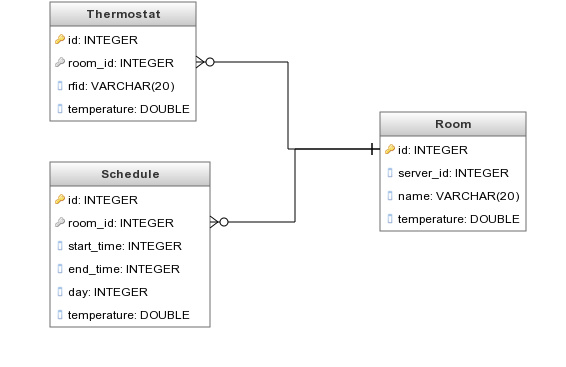
\includegraphics[width=0.8\textwidth]{images/mobile_database.jpeg}
	\end{center}
	\caption{The database model used in the mobile application.}
	\label{fig:db_model}
\end{figure}

After the initial setup of the database, the user is confronted with four questions about his daily routine. The questions are:

\begin{itemize}
\item{When do you usually wake up in the morning?}
\item{When do you usually leave for work in the morning?}
\item{When do you usually get home from work in the evening?}
\item{When do you usually go to bed in the evening?}
\end{itemize}

\begin{figure}
	\begin{center}
		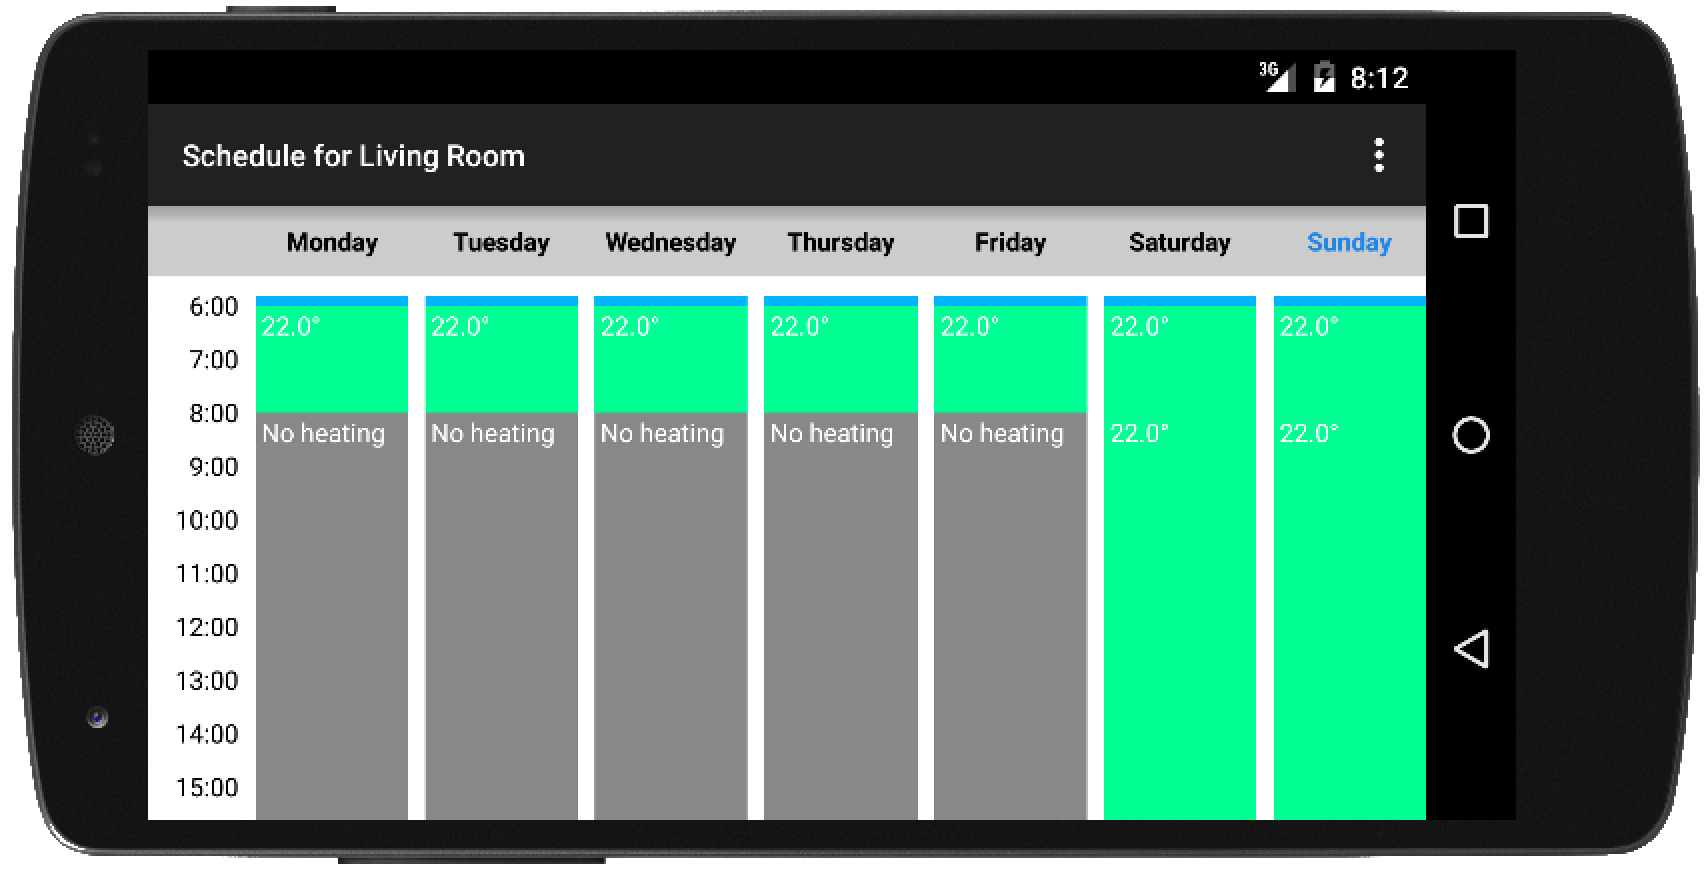
\includegraphics[width=0.8\textwidth]{images/default_heating_schedule.png}
	\end{center}
	\caption{A sample default heating schedule after the initial setup of the system.}
	\label{fig:default_schedulel}
\end{figure}

With the help of these four questions the application is able to set up a default heating schedule which is initially used for all the rooms that are added in the future. It simply takes the answers to the four questions and sets up the heating schedule in the following way: 

\begin{itemize}
\item{If the user is at home, the temperature is set to the default value for when somebody is at home.}
\item{If the user is at work, the heating is turned off completely.}
\item{If the user is sleeping, the temperature is set to the default value for the night.}
\item{On weekends, the temperature stays on the default value for being home throughout the whole day.}
\end{itemize}

These default values are initially set to 16 and 22 degrees celsius for being home and sleeping respectively. These values can be changed in the settings menu from the home view (Section \ref{sec:home_view}).

If desired, the user can also change every heating schedule separately to his own needs. More details about heating schedules can be found in Section \ref{sec:schedule_view}.

\subsection{The Home View}
\label{sec:home_view}
The home view is where the application usually starts after successful registration of the raspberry pi with the server. In the home view the user can see all the rooms he added to the system with the corresponding current temperatures in each room. The colour of the tiles with the room names are also an indicator to how hot the room is in its current state, ranging from blue (cold) to green (normal) to red (hot). Clicking one of the tiles will lead the user to the room detail view described in Section \ref{sec:detail_view}. Next to the current temperature of each room there is an optional flame icon indicating that the room is being heated up at the moment. See Figure \ref{fig:home_view} for an example.

Via the menu in the upper righthand corner, the user can choose to add new rooms or delete existing ones. Adding a new room simply requires a new name for the room to be entered. After the creation of a new room the user is immediately transferred to the room detail view so that he can add new thermostats to the room. For more details about the room detail view see Section \ref{sec:detail_view}.

\begin{figure}
	\begin{center}
		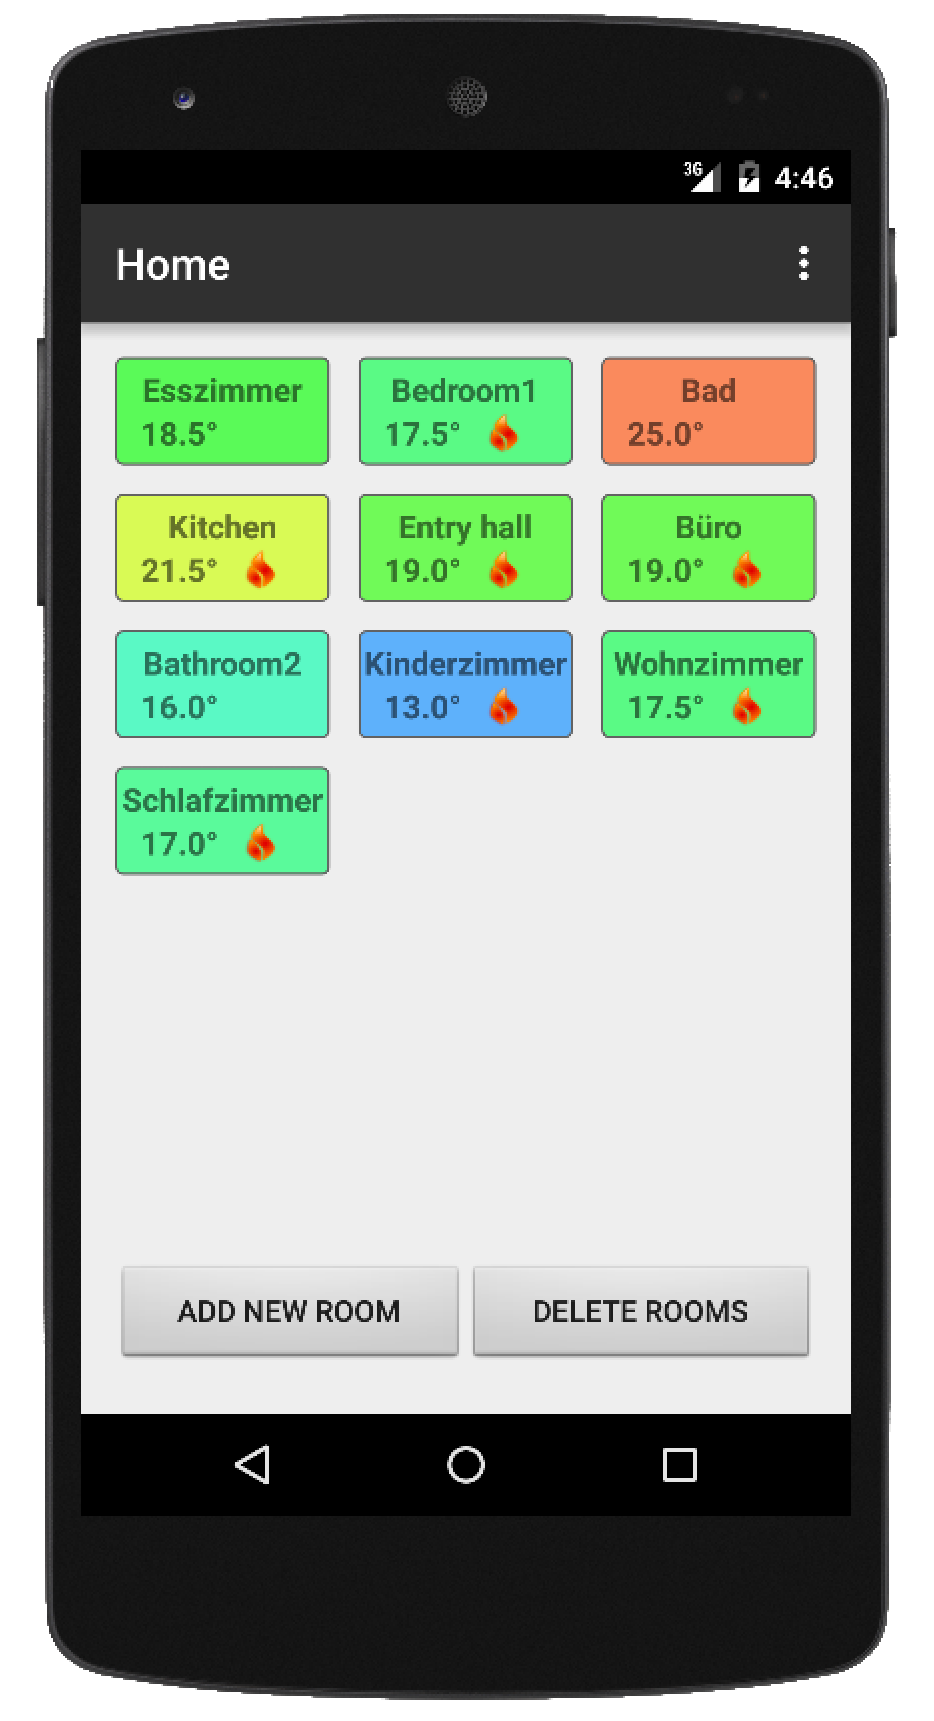
\includegraphics[width=0.8\textwidth]{images/home_view.png}
	\end{center}
	\caption{A sample home view with some random rooms.}
	\label{fig:home_view}
\end{figure}

\subsection{The Room Detail View}
\label{sec:detail_view}
After clicking one of the tiles in the home view the user is presented with more details about the room. He can see a list with all the thermostats, the current temperature in the room indicated with a large thermometer and also a slider next to it for adjusting the desired temperature of the room.

The desired temperature comes from the heating schedule currently active for the room. If the user wants to change the desired temperature he can simply drag the slider to a new position. The heating schedule for the room will be adjusted automatically as well.

If the user wants to change the heating schedule manually he can do so by selecting "View/Edit schedule" from the menu located in the upper righthand corner. This will lead him to the schedule view described further in Section \ref{sec:schedule_view}. 
\todo{picture detail view}

\subsection{The Schedule View}
\label{sec:schedule_view}
\label{sec:last_view}
The schedule view shows the heating schedule of the room the user has selected previously in the home view. The application is forced into landscape mode to be able to display all the days of the week. The current day of the week is highlighted for easier usability. The user can scroll up and down to see all the different times of the day. 

Adding a new entry is simple: with a single tap anywhere on the schedule the user can add a new entry in the corresponding time slot. He can also adjust the exact times of the new entry after tapping. After providing the desired target temperature for the new entry the user can confirm the data and the new schedule entry is sent to the local database as well as the online server right away. 

Removing a heating schedule entry is not possible and should not be necessary. If the user wants to turn off the heating for a certain period he can simply add a new entry and check the "No heating" checkbox. See Figure \ref{fig:new_schedule_entry} for an example.

\begin{figure}
	\begin{center}
		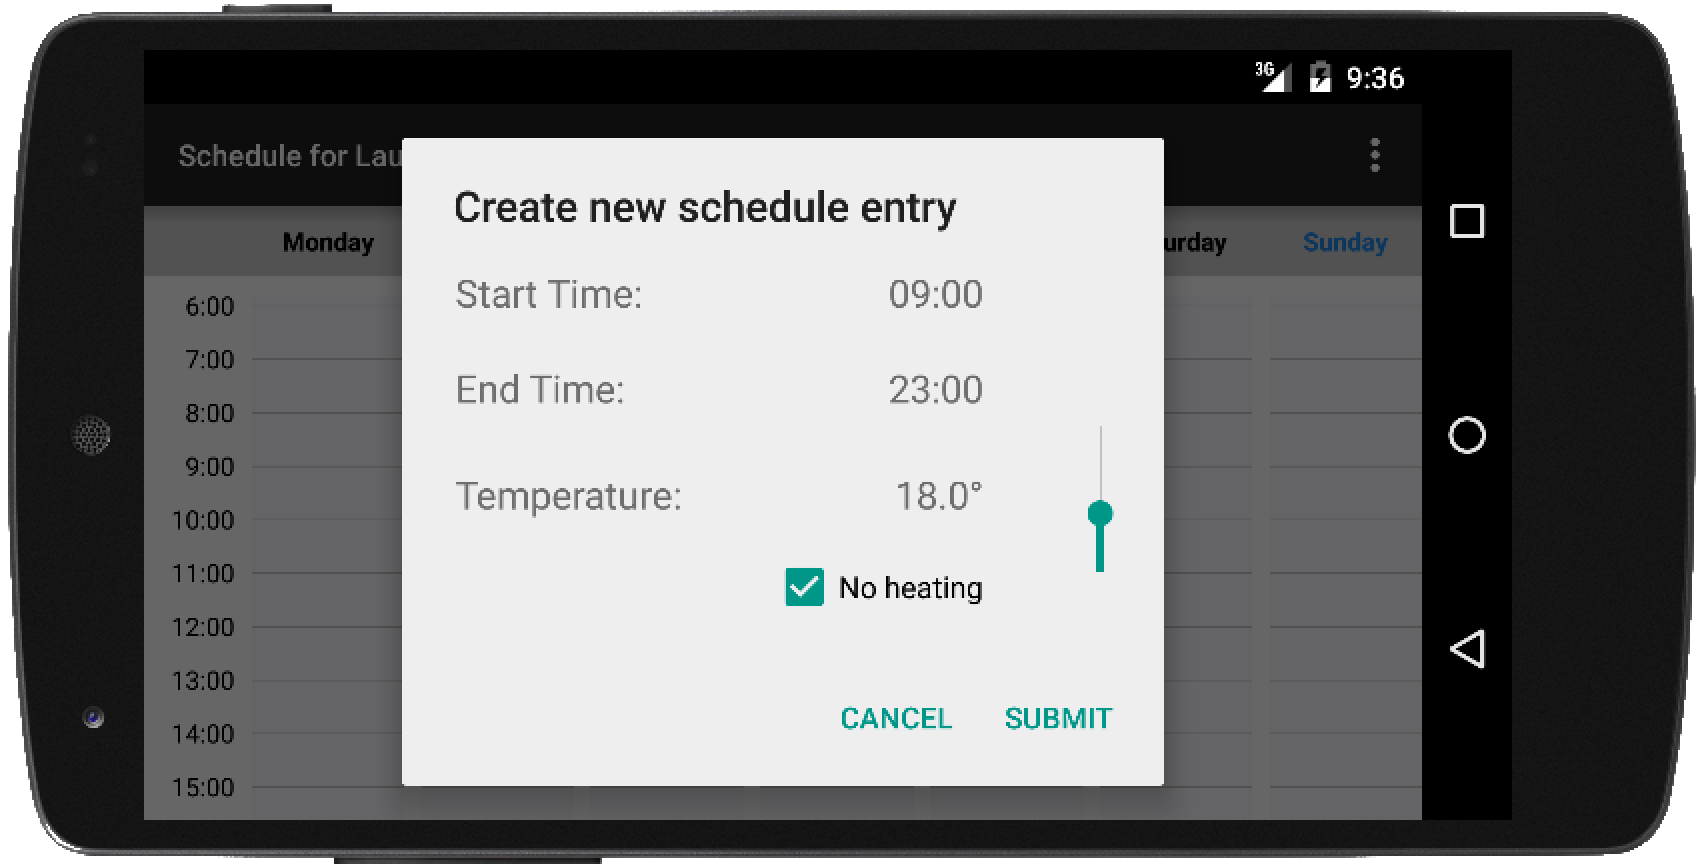
\includegraphics[width=0.8\textwidth]{images/new_schedule_entry.png}
	\end{center}
	\caption{The popup for adding a new heating schedule entry.}
	\label{fig:new_schedule_entry}
\end{figure}

\section{Evaluation}

\subsection {Use cases coverage}
Our mobile control application covers most of the use cases introduced in Section \ref{sec:use_cases} adequately. As shown later in some cases we decided to either leave the feature out for simplicity's sake or because it was out of scope for this lab project.

\begin{enumerate}
\item \textbf{Use Case: User wants to install the system}

Covered by the welcome view: The user can easily setup the system using the NFC tags distributed on the raspberry pi and the thermostats with the help of the information displayed on the application.
\item \textbf{Use Case: User feels cold}

Covered by the detail view: The user can adjust the temperature of the room he is currently in using the slider in the detail view.
\item \textbf{Use Case: User wants to save money}

Indirectly covered: The user can choose to set the default temperatures to values lower than usual in order to save money.
\item \textbf{Use Case: User wants to add a room to an existing system}

Covered by the home view: The user can simply add a room using the menu in the upper righthand corner.
\item \textbf{Use Case: User wants to add a thermostat to a room in the system}

Covered by the detail view: The user can add a new thermostat to the currently selected room by simply scanning its NFC tag.
\item \textbf{Use Case: User feels hot}

Covered by the detail view: The user can adjust the temperature of the room he is currently in using the slider in the detail view.
\end{enumerate}

\subsection{User study}
We have conducted a user study with some of our fellow students. Here are some of their comments about the usability and the application's design.

\todo{Actually do it...}
%!TEX root = ../thesis.tex

\chapter{Evaluation}
\label{sec:evaluation}

In this section we will evaluate our set design goals and discuss our implementation in detail.
Further we will analyze our design decisions.
Where applicable the functional and non-functional requirements will be validated.

\section{Infrastructure}

This section follows the same structure as used in the previous Chapter~\ref{sec:infrastructure}.
The infrastructure consists of the server part and the local part.
Both are evaluated in the following sections.

\subsection{Server Infrastructure}

\subsubsection{Design Goals}

Section~\ref{sec:server_infrastructure_design_goals} lists the design goals defined for this project part.
Each design goal will be evaluated in a separate paragraph below.

\paragraph{Modularity and Extensibility} Django emphasizes reusability of components.
This solid background allows us to clearly separate different concerns to achieve modularity.
Further the distinct components simplify application extensions by easily adding new resources, representations, views or URLs.

% TODO add some examples?

\paragraph{Usability} In order for a developer to be able to familiarize himself with a new API it is important to provide clear documentation and a platform to use the API.
The browsable API as described in Section~\ref{sec:server_infrastructure_restful_api} provides both.
It allows a developer to interactively explore the resource structure by navigating the hyperlinked URLs.
The browsable API also provides easy interaction possibilities to create, read, update and delete resources.
Further the API describes the allowed methods when requesting a particular resource.
One of these methods named \emph{OPTIONS} additionally shows fields and their requirements.

\paragraph{Testability}

The modular program structure and the chosen Django framework support the creation and automatized execution of software tests.
These automatized tests are continuously executed on a hosted service and show that the tests run regularly and successfully.

\todo[inline]{Siehe auch Report Structure.}


\subsubsection{Design Decisions}

During the system implementation a few design decisions were chosen and will be evaluated in the following paragraphs.

\paragraph{Nested URL schema}

The model hierarchy is represented using a nested URL schema.
This schema suits the model structure in tree form and induces good readable URLs.
Django is designed for flat URLs but is still flexible enough to support the design decision of nested resources represented within the URL.

\paragraph{Resource identifier as the first field}

Within the resource representation the resource identifier is always the first field.
This allows to easily recognize the identifier within resource representations and especially within nested resource representation.

\paragraph{Resource referencing}

Resources are referenced by including their representation.
This design decision improves the usability of the API, as related resources are shown in their full representation.
In contrast collections are referenced via their URL.
This is necessary to limit the representation size and avoid infinite recursions.
For example in a parent-child relationship the child representation contains the representation of its parent.
The parent representation itself contains the collection representation of its children.
Therefore the collection representation cannot contain the full representations of its resources.

\paragraph{Identification of URL fields}

Fields representing a URL are identified by the name \highlight{url} or the suffix \highlight{\_url}.
This design decision facilitates the recognition of hyperlinks which also allows an automatized navigation through the API.



\subsection{Local Deployment}


%\subsubsection{Design Goals}

The following section will evaluate each of the design goals defined in Section~\ref{sec:local_infrastructure_design_goals}.

The local infrastructure section is about the implementation part done on the residential communication gateway.
Therefore the following paragraphs focus on the evaluation of software running on the Raspberry computer.

\subsubsection{Performance}
% for low computational effort and power consumption on embedded systems.

The system performance depends on two aspects.
First, the software part.
The programming language \emph{Python} was chosen at it is suitable for developing on embedded hardware with possibly long-running input/output operations.
Another important component is the system design of independent scripts triggered by the scheduler \emph{cron}.
Second, the embedded hardware part.
The chosen hardware needs to be powerful enough to run the software implementation.

For evaluation of the ratio between required software performance and provided hardware performance the CPU load is monitored.
We use the \emph{sar} command from the \emph{apt-get} package \emph{sysstat} to analyze the average CPU utilization.
Over a period of seven days of regular system runtime the average CPU load was 0.28 percent.
This indicates that the hardware is powerful enough to run the designed software implementation.


\subsubsection{Robustness}
% to let the system behave reasonably in presence of failures, especially connection problems.

We defined robustness to be the ability of the system to behave reasonably in the presence of failures, especially connection problems.
The local communication gateway is designed as two independent tasks.
The first task is the retrieval and storage of the temperature data and the application of the defined schedule.
The second task is the synchronization of the local data storage with the remote web server.
This design splits the "Aufgabenbereich" of the local communication system into two simpler separated tasks with a clearly defined interface, the local data storage.
In the presence of a failure only one of the two tasks is affected whereas the other task is still able continue its purpose.

For example in the event of a temporary internet connection disruption the system will keep operating the last downloaded heating schedule and store the temperature history.
After the disruption the local data storage is synchronized and the system continues to operate on the most actual settings.

Another failure scenario would be the temporary disconnection of a wireless thermostat.
In such a case the non-affected thermostats are still functional and the heating schedule of all thermostats is kept synchronized.
As soon as the system reestablishes the connection to the affected thermostat the system continues to work as planned.
In the meantime neither the properly operating thermostats nor the synchronization of all thermostats' heating schedules is impaired.


\subsubsection{Reliability}
% for a high probability that the system operates as expected

In order to check the reliability of the system in a real world scenario the system has been deployed in a residential home.
Previous work in this area compared the defined room temperatures with the actual room temperatures to conclude on the proper work of a heating system\cite{eigenmann2012opportunisticSensing}.
Due to the season and the according temperatures this evaluation is not possible for this project.
Instead we focus on the communication between the wireless thermostats, the local communication gateway and the remote server.

The main data sources for our analysis are the generated log files and databases on the local communication gateway.

On the local communication gateway there are data sources: the log files written by two scripts and the local storage used to cache the temperature readings and other meta information.
If not stated otherwise, the data from the time span of August 2015 is used for the following evaluations.

\paragraph{Analysis of the local data storage}

% 2969 Rows returned from: SELECT * FROM heating_temperature
% WHERE timestamp BETWEEN '2015-08-01' AND '2015-09-01' (took 12ms)

% SELECT strftime('%d', timestamp), COUNT(*), * FROM heating_temperature
% WHERE timestamp BETWEEN '2015-08-01' AND '2015-09-01'
% GROUP BY strftime('%d', timestamp)
We start with the analysis of the local data storage.
The local communication gateway queries the thermostats every 15 minutes, i.e. 96 times a day.
The maximal number of temperature measurements and meta entries would therefore be 2976 for the whole month of August.
The local data storage contains 2969 of these recorded temperature measurements in this date range, resulting in a coverage of 99.76 percent.
See Table~\ref{table:evaluation_local_database_coverage} for the full coverage data.

\begin{table}
	\begin{center}
		\begin{tabular}{ l | r r r }
			Local Database entries & Maximal count & Actual count & Coverage \\
			\hline
			Temperature					& 2976 & 2969 & 99.76 \% \\
%			Server temperature entries	& 2976 & 2969 & 99.76 \%
			Meta information			& 2976 & 2970 & 99.80 \% \\
		\end{tabular}
		\caption{Retrieved temperature measurements and meta entries in a real world deployment in August 2015.}
		\label{table:evaluation_local_database_coverage}
	\end{center}
\end{table}

\paragraph{Analysis of the local log files}

Each log entry has a severity level indicating how important a log event is in terms of system functionality and reliability.
We analyze these severity levels and their according log messages to show the intended system behavior as well as to identify potential problems.



\todo[inline]{move the server part out of the local part}


The evaluation of the remote web server is similar to the analysis of the local database and log files.

\paragraph{Analysis of the server database}


% 2969 Rows returned from: SELECT * FROM smart_heating_temperature WHERE thermostat_id = "04B753B9212580"
% AND datetime BETWEEN '2015-08-01' AND '2015-09-01' (took 23ms)
The analysis of the server database is similar to the analysis of the local database.
In the evaluated time span there are 2969 temperature entries out of 2976 possible measurements.
These are the same entries as on the local communication gateway and shows that all measurements were successfully transmitted to the server.

\paragraph{Analysis of the server log files}

The server logs all received requests into a log file.
Each log entry contains the requested URL, the HTTP method and the HTTP response code.
We analyze all requests to any temperature resource.
In the chosen time span here were 2969 POST requests each adding a single temperature measurement.
This matches the number of temperature entries in the database.






\paragraph{Interoperability}
% to cooperate with other distributed systems

We define interoperability as the system's ability to cooperate with other distributed systems.
The whole infrastructure is designed to communicate according to recognized open standards and architectural styles such as \emph{Constrained Application Protocol (CoAP)}, \emph{Hypertext Transfer Protocol (HTTP)}, \emph{Internet Protocol (IP)}, \emph{JavaScript Object Notation (JSON)} and \emph{Representational State Transfer (REST)}.
This way the developed infrastructure is able to cooperate with other distributed system via the defined interfaces.










\section{Mobile App}

%!TEX root = ../thesis.tex

\chapter{Future Work}
\label{sec:futurework}

%Anything that is interesting -- but you did not have the time to pursue -- fits into future work.

In the scope of this lab project we developed a reliable heating control infrastructure and the corresponding innovative mobile application.
We focused these implementations to build a solid basis for future projects to build upon.
In the following we outline a few interesting ideas that we did not have the time to pursue but that could be implemented as a future work.

%The developed Web server builds a solid tested framework that stores and processes the collected data.
The developed system could be extended to track and predict user locations.
This would allow to dynamically adjust the heating schedule to react to spontaneous user behavior deviations and could further decrease the energy consumption and increase the users comfort level in certain cases.

As a part of this project we implemented a mobile application designed for Android smart phones.
Another possibility for future work would be an additional user interface that could show more complex data analysis suitable for devices with bigger screens.

\todo[inline]{SAMUEL: Future work mobile application}

%!TEX root = ../thesis.tex

\chapter{Conclusion}
\label{sec:conclusion}

Give a summary on what you did and what the major results are.

\bibliographystyle{abbrv}
\bibliography{references}

%\listoffigures
\appendix
%!TEX root = ../thesis.tex

\chapter{First Appendix}
\label{sec:first_appendix}

Use appendix for more anything that does not fit into the main document (e.g., implementation details).

\todo[inline]{Include links to all GitHub repos}

\todo[inline]{insert protocol}
\parskip 0pt

\end{document}
